\documentclass[]{article}
\usepackage{lmodern}
\usepackage{amssymb,amsmath}
\usepackage{ifxetex,ifluatex}
\usepackage{fixltx2e} % provides \textsubscript
\ifnum 0\ifxetex 1\fi\ifluatex 1\fi=0 % if pdftex
  \usepackage[T1]{fontenc}
  \usepackage[utf8]{inputenc}
\else % if luatex or xelatex
  \ifxetex
    \usepackage{mathspec}
  \else
    \usepackage{fontspec}
  \fi
  \defaultfontfeatures{Ligatures=TeX,Scale=MatchLowercase}
\fi
% use upquote if available, for straight quotes in verbatim environments
\IfFileExists{upquote.sty}{\usepackage{upquote}}{}
% use microtype if available
\IfFileExists{microtype.sty}{%
\usepackage{microtype}
\UseMicrotypeSet[protrusion]{basicmath} % disable protrusion for tt fonts
}{}
\usepackage[margin=1in]{geometry}
\usepackage{hyperref}
\hypersetup{unicode=true,
            pdftitle={Final Project For Regression Analysis},
            pdfauthor={ChenXG 陈栩淦 3160104014},
            pdfborder={0 0 0},
            breaklinks=true}
\urlstyle{same}  % don't use monospace font for urls
\usepackage{color}
\usepackage{fancyvrb}
\newcommand{\VerbBar}{|}
\newcommand{\VERB}{\Verb[commandchars=\\\{\}]}
\DefineVerbatimEnvironment{Highlighting}{Verbatim}{commandchars=\\\{\}}
% Add ',fontsize=\small' for more characters per line
\usepackage{framed}
\definecolor{shadecolor}{RGB}{248,248,248}
\newenvironment{Shaded}{\begin{snugshade}}{\end{snugshade}}
\newcommand{\KeywordTok}[1]{\textcolor[rgb]{0.13,0.29,0.53}{\textbf{#1}}}
\newcommand{\DataTypeTok}[1]{\textcolor[rgb]{0.13,0.29,0.53}{#1}}
\newcommand{\DecValTok}[1]{\textcolor[rgb]{0.00,0.00,0.81}{#1}}
\newcommand{\BaseNTok}[1]{\textcolor[rgb]{0.00,0.00,0.81}{#1}}
\newcommand{\FloatTok}[1]{\textcolor[rgb]{0.00,0.00,0.81}{#1}}
\newcommand{\ConstantTok}[1]{\textcolor[rgb]{0.00,0.00,0.00}{#1}}
\newcommand{\CharTok}[1]{\textcolor[rgb]{0.31,0.60,0.02}{#1}}
\newcommand{\SpecialCharTok}[1]{\textcolor[rgb]{0.00,0.00,0.00}{#1}}
\newcommand{\StringTok}[1]{\textcolor[rgb]{0.31,0.60,0.02}{#1}}
\newcommand{\VerbatimStringTok}[1]{\textcolor[rgb]{0.31,0.60,0.02}{#1}}
\newcommand{\SpecialStringTok}[1]{\textcolor[rgb]{0.31,0.60,0.02}{#1}}
\newcommand{\ImportTok}[1]{#1}
\newcommand{\CommentTok}[1]{\textcolor[rgb]{0.56,0.35,0.01}{\textit{#1}}}
\newcommand{\DocumentationTok}[1]{\textcolor[rgb]{0.56,0.35,0.01}{\textbf{\textit{#1}}}}
\newcommand{\AnnotationTok}[1]{\textcolor[rgb]{0.56,0.35,0.01}{\textbf{\textit{#1}}}}
\newcommand{\CommentVarTok}[1]{\textcolor[rgb]{0.56,0.35,0.01}{\textbf{\textit{#1}}}}
\newcommand{\OtherTok}[1]{\textcolor[rgb]{0.56,0.35,0.01}{#1}}
\newcommand{\FunctionTok}[1]{\textcolor[rgb]{0.00,0.00,0.00}{#1}}
\newcommand{\VariableTok}[1]{\textcolor[rgb]{0.00,0.00,0.00}{#1}}
\newcommand{\ControlFlowTok}[1]{\textcolor[rgb]{0.13,0.29,0.53}{\textbf{#1}}}
\newcommand{\OperatorTok}[1]{\textcolor[rgb]{0.81,0.36,0.00}{\textbf{#1}}}
\newcommand{\BuiltInTok}[1]{#1}
\newcommand{\ExtensionTok}[1]{#1}
\newcommand{\PreprocessorTok}[1]{\textcolor[rgb]{0.56,0.35,0.01}{\textit{#1}}}
\newcommand{\AttributeTok}[1]{\textcolor[rgb]{0.77,0.63,0.00}{#1}}
\newcommand{\RegionMarkerTok}[1]{#1}
\newcommand{\InformationTok}[1]{\textcolor[rgb]{0.56,0.35,0.01}{\textbf{\textit{#1}}}}
\newcommand{\WarningTok}[1]{\textcolor[rgb]{0.56,0.35,0.01}{\textbf{\textit{#1}}}}
\newcommand{\AlertTok}[1]{\textcolor[rgb]{0.94,0.16,0.16}{#1}}
\newcommand{\ErrorTok}[1]{\textcolor[rgb]{0.64,0.00,0.00}{\textbf{#1}}}
\newcommand{\NormalTok}[1]{#1}
\usepackage{graphicx,grffile}
\makeatletter
\def\maxwidth{\ifdim\Gin@nat@width>\linewidth\linewidth\else\Gin@nat@width\fi}
\def\maxheight{\ifdim\Gin@nat@height>\textheight\textheight\else\Gin@nat@height\fi}
\makeatother
% Scale images if necessary, so that they will not overflow the page
% margins by default, and it is still possible to overwrite the defaults
% using explicit options in \includegraphics[width, height, ...]{}
\setkeys{Gin}{width=\maxwidth,height=\maxheight,keepaspectratio}
\IfFileExists{parskip.sty}{%
\usepackage{parskip}
}{% else
\setlength{\parindent}{0pt}
\setlength{\parskip}{6pt plus 2pt minus 1pt}
}
\setlength{\emergencystretch}{3em}  % prevent overfull lines
\providecommand{\tightlist}{%
  \setlength{\itemsep}{0pt}\setlength{\parskip}{0pt}}
\setcounter{secnumdepth}{5}
% Redefines (sub)paragraphs to behave more like sections
\ifx\paragraph\undefined\else
\let\oldparagraph\paragraph
\renewcommand{\paragraph}[1]{\oldparagraph{#1}\mbox{}}
\fi
\ifx\subparagraph\undefined\else
\let\oldsubparagraph\subparagraph
\renewcommand{\subparagraph}[1]{\oldsubparagraph{#1}\mbox{}}
\fi

%%% Use protect on footnotes to avoid problems with footnotes in titles
\let\rmarkdownfootnote\footnote%
\def\footnote{\protect\rmarkdownfootnote}

%%% Change title format to be more compact
\usepackage{titling}

% Create subtitle command for use in maketitle
\newcommand{\subtitle}[1]{
  \posttitle{
    \begin{center}\large#1\end{center}
    }
}


\renewcommand{\contentsname}{目录}
\renewcommand{\abstractname}{}
\usepackage{setspace}

\usepackage[BoldFont,SlantFont]{xeCJK}
\setmainfont{Times New Roman}
\setCJKmainfont[ItalicFont={STKaiti}, BoldFont={STHeiti}]{STKaiti}
\setCJKmonofont{STKaiti} % 设置缺省中文字体
\linespread{1.5}    % 设置行间距
\parindent 2em  % 设置段首缩进

%
%==================================================================================================

\setlength{\droptitle}{-2em}

  \title{
    King County房屋销售价格案例分析 \\
    {\Large ——Final Project For Regression Analysis}
  }
    \pretitle{\vspace{\droptitle}\centering\huge}
  \posttitle{\par}
    \author{
      陈栩淦 3160104014 \\
      数学科学学院
    }
    \preauthor{\centering\large\emph}
  \postauthor{\par}
      \predate{\centering\large\emph}
  \postdate{\par}
    \date{12/19/2018}






%
%==================================================================================================


\begin{document}

\begin{figure}[!htbp]
\centering

\includegraphics[width =0.7\linewidth]{FinalProjectForRegressionAnalysis_files/figure-latex/first1.png}
\end{figure}

\begin{figure}[!htbp]
\centering

\includegraphics[width =0.6\linewidth]{FinalProjectForRegressionAnalysis_files/figure-latex/first2.png}
\end{figure}

~\\

\begin{table}[!htbp]
\centering
{\large
\begin{tabular}{rc}
课程名称: & 回归分析 \\ \\
报告题目: & King County房屋销售价格案例分析 \\  \\
指导老师: & 庞天晓 \\ \\
学\quad \quad 院: & 数学科学学院 \\ \\
专\quad \quad 业: & 数学与应用数学(金融学交叉创新平台)\\ \\
姓名学号: & 陈栩淦\quad 3160104014 
\end{tabular}
} 
\end{table}

\thispagestyle{empty}


%
%==================================================================================================


\maketitle

\begin{abstract} 
{\large
\textbf{【摘要】\ }  本报告是King County(包括Seattle)的房屋销售价格的案例分析,来源于Kaggle的Datasets,其中包括了2014年5月到2015年5月的房屋销售情况(价格数据和18个房屋特征),在分析过程中选取了其中300个样本点。报告首先对数据进行了回归诊断(包括模型、数据和多重共线性的诊断),其次分别进行了线性回归(变量选择)、主成分回归和岭回归分析,并进行预测。此外,本报告还拓展了其他内容,包括resample方法(Boostrap和Cross-Validation)和Elastic net方法。
\footnote{注:为了减少文章篇幅,本报告PDF文件中的代码只展示了必要的代码,而结果是直接运行得到。如若要看完整代码,可以查看同文件夹中的.Rmd或者.html文件。此外,本报告中所有带有随机性的过程均设随机种子为123.}
}
\end{abstract}


\setcounter{page}{0}
\thispagestyle{empty}



\newpage
\tableofcontents
\newpage



%
%==================================================================================================

首先定义运行环境空间,并加载相关的packages。
\begin{Shaded}
\begin{Highlighting}[]
\KeywordTok{Sys.setlocale}\NormalTok{(}\StringTok{"LC_ALL"}\NormalTok{, }\DataTypeTok{locale =} \StringTok{"en_US.UTF-8"}\NormalTok{)}
\KeywordTok{setwd}\NormalTok{(}\StringTok{"~/Project/RegressionAnalysis"}\NormalTok{)}

\KeywordTok{library}\NormalTok{(reshape2)  }\CommentTok{# for melt}
\KeywordTok{library}\NormalTok{(GGally)  }\CommentTok{# for ggpairs}
\KeywordTok{library}\NormalTok{(car)  }\CommentTok{# for outlierTest}
\KeywordTok{library}\NormalTok{(DAAG)  }\CommentTok{# for vif, eigen and kappa}
\KeywordTok{library}\NormalTok{(leaps)  }\CommentTok{# for leaps and regsubsets}
\KeywordTok{library}\NormalTok{(DAAG)  }\CommentTok{# for press}
\KeywordTok{library}\NormalTok{(SignifReg)  }\CommentTok{# for SignifReg}
\KeywordTok{library}\NormalTok{(boot)  }\CommentTok{# for lm.boot and cv.glm}
\KeywordTok{library}\NormalTok{(MASS)  }\CommentTok{# for lm.ridge}
\KeywordTok{library}\NormalTok{(glmnet) }\CommentTok{# for glmnet and cv.glmnet}
\KeywordTok{library}\NormalTok{(ggplot2)}
\end{Highlighting}
\end{Shaded}




%
%==================================================================================================


\section{数据集}





%
%--------------------------------------------------------------------------------------------------
\subsection{数据说明及来源}

本报告所用数据为King
County(包括Seattle)的房屋销售价格,其中包括了从2014年5月到2015年5月的房屋销售情况,总共有21613个样本点。其中数据来源为Kaggle/Datasets/House Sales in King County, USA,\\
网址为https://www.kaggle.com/harlfoxem/housesalesprediction。下面为网站上该数据集的描述。

\begin{quote}
\begin{itemize}
\tightlist
\item
  Overview
\end{itemize}

This dataset contains house sale prices for King County, which includes
Seattle. It includes homes sold between May 2014 and May 2015.

It's a great dataset for evaluating simple regression models.

\begin{itemize}
\tightlist
\item
  about this file
\end{itemize}

19 house features plus the price and the id columns, along with 21613
observations.
\end{quote}




\subsubsection{数据信息}

该数据包括了房屋id、销售时间和销售价格的基本信息:

\begin{itemize}
\tightlist
\item
  id: a notation for a house
\item
  date: Date house was sold
\item
  price: Price is prediction target
\end{itemize}

以及18个房屋特征features,如下:

\begin{itemize}
\tightlist
\item
  bedrooms: Number of Bedrooms/House
\item
  bathrooms: Number of bathrooms/House
\item
  sqft\_living: square footage of the home
\item
  sqft\_lot: square footage of the lot
\item
  floors: Total floors (levels) in house
\item
  waterfront: House which has a view to a waterfront
\item
  view: Has been viewed
\item
  condition: How good the condition is ( Overall )
\item
  grade: overall grade given to the housing unit, based on King County
  grading system
\item
  sqft\_above: square footage of house apart from basement
\item
  sqft\_basement: square footage of the basement
\item
  yr\_built: Built Year
\item
  yr\_renovated: Year when house was renovated
\item
  zipcode: zip
\item
  lat: Latitude coordinate
\item
  long: Longitude coordinate
\item
  sqft\_living15: Living room area in 2015(implies-- some renovations)
  This might or might not have affected the lotsize area
\item
  sqft\_lot15: lotSize area in 2015(implies-- some renovations)
\end{itemize}







%
%--------------------------------------------------------------------------------------------------
\subsection{读取数据}

首先读取数据,该文件``kc\_house\_data.csv''为直接下载得到。下面查看数据结构。

\begin{Shaded}
\begin{Highlighting}[]
\KeywordTok{str}\NormalTok{(data)}
\end{Highlighting}
\end{Shaded}

\begin{verbatim}
## 'data.frame':    21613 obs. of  20 variables:
##  $ id           : num  7.13e+09 6.41e+09 5.63e+09 2.49e+09 1.95e+09 ...
##  $ date         : Factor w/ 372 levels "20140502T000000",..: 165 221 291 221 284 11 57 252 340 306 ...
##  $ price        : num  221900 538000 180000 604000 510000 ...
##  $ bedrooms     : int  3 3 2 4 3 4 3 3 3 3 ...
##  $ bathrooms    : num  1 2.25 1 3 2 4.5 2.25 1.5 1 2.5 ...
##  $ sqft_living  : int  1180 2570 770 1960 1680 5420 1715 1060 1780 1890 ...
##  $ sqft_lot     : int  5650 7242 10000 5000 8080 101930 6819 9711 7470 6560 ...
##  $ floors       : num  1 2 1 1 1 1 2 1 1 2 ...
##  $ waterfront   : int  0 0 0 0 0 0 0 0 0 0 ...
##  $ view         : int  0 0 0 0 0 0 0 0 0 0 ...
##  $ condition    : int  3 3 3 5 3 3 3 3 3 3 ...
##  $ grade        : int  7 7 6 7 8 11 7 7 7 7 ...
##  $ sqft_above   : int  1180 2170 770 1050 1680 3890 1715 1060 1050 1890 ...
##  $ yr_built     : int  1955 1951 1933 1965 1987 2001 1995 1963 1960 2003 ...
##  $ yr_renovated : int  0 1991 0 0 0 0 0 0 0 0 ...
##  $ zipcode      : int  98178 98125 98028 98136 98074 98053 98003 98198 98146 98038 ...
##  $ lat          : num  47.5 47.7 47.7 47.5 47.6 ...
##  $ long         : num  -122 -122 -122 -122 -122 ...
##  $ sqft_living15: int  1340 1690 2720 1360 1800 4760 2238 1650 1780 2390 ...
##  $ sqft_lot15   : int  5650 7639 8062 5000 7503 101930 6819 9711 8113 7570 ...
\end{verbatim}


下面查看数据的描述性统计特征

\begin{Shaded}
\begin{Highlighting}[]
\KeywordTok{summary}\NormalTok{(data)}
\end{Highlighting}
\end{Shaded}

\begin{verbatim}
##        id                         date           price        
##  Min.   :1.000e+06   20140623T000000:  142   Min.   :  75000  
##  1st Qu.:2.123e+09   20140625T000000:  131   1st Qu.: 321950  
##  Median :3.905e+09   20140626T000000:  131   Median : 450000  
##  Mean   :4.580e+09   20140708T000000:  127   Mean   : 540088  
##  3rd Qu.:7.309e+09   20150427T000000:  126   3rd Qu.: 645000  
##  Max.   :9.900e+09   20150325T000000:  123   Max.   :7700000  
##                      (Other)        :20833                    
##     bedrooms        bathrooms      sqft_living       sqft_lot      
##  Min.   : 0.000   Min.   :0.000   Min.   :  290   Min.   :    520  
##  1st Qu.: 3.000   1st Qu.:1.750   1st Qu.: 1427   1st Qu.:   5040  
##  Median : 3.000   Median :2.250   Median : 1910   Median :   7618  
##  Mean   : 3.371   Mean   :2.115   Mean   : 2080   Mean   :  15107  
##  3rd Qu.: 4.000   3rd Qu.:2.500   3rd Qu.: 2550   3rd Qu.:  10688  
##  Max.   :33.000   Max.   :8.000   Max.   :13540   Max.   :1651359  
##                                                                    
##      floors        waterfront            view          condition    
##  Min.   :1.000   Min.   :0.000000   Min.   :0.0000   Min.   :1.000  
##  1st Qu.:1.000   1st Qu.:0.000000   1st Qu.:0.0000   1st Qu.:3.000  
##  Median :1.500   Median :0.000000   Median :0.0000   Median :3.000  
##  Mean   :1.494   Mean   :0.007542   Mean   :0.2343   Mean   :3.409  
##  3rd Qu.:2.000   3rd Qu.:0.000000   3rd Qu.:0.0000   3rd Qu.:4.000  
##  Max.   :3.500   Max.   :1.000000   Max.   :4.0000   Max.   :5.000  
##                                                                     
##      grade          sqft_above      yr_built     yr_renovated   
##  Min.   : 1.000   Min.   : 290   Min.   :1900   Min.   :   0.0  
##  1st Qu.: 7.000   1st Qu.:1190   1st Qu.:1951   1st Qu.:   0.0  
##  Median : 7.000   Median :1560   Median :1975   Median :   0.0  
##  Mean   : 7.657   Mean   :1788   Mean   :1971   Mean   :  84.4  
##  3rd Qu.: 8.000   3rd Qu.:2210   3rd Qu.:1997   3rd Qu.:   0.0  
##  Max.   :13.000   Max.   :9410   Max.   :2015   Max.   :2015.0  
##                                                                 
##     zipcode           lat             long        sqft_living15 
##  Min.   :98001   Min.   :47.16   Min.   :-122.5   Min.   : 399  
##  1st Qu.:98033   1st Qu.:47.47   1st Qu.:-122.3   1st Qu.:1490  
##  Median :98065   Median :47.57   Median :-122.2   Median :1840  
##  Mean   :98078   Mean   :47.56   Mean   :-122.2   Mean   :1987  
##  3rd Qu.:98118   3rd Qu.:47.68   3rd Qu.:-122.1   3rd Qu.:2360  
##  Max.   :98199   Max.   :47.78   Max.   :-121.3   Max.   :6210  
##                                                                 
##    sqft_lot15    
##  Min.   :   651  
##  1st Qu.:  5100  
##  Median :  7620  
##  Mean   : 12768  
##  3rd Qu.: 10083  
##  Max.   :871200  
## 
\end{verbatim}


\subsubsection{划分训练集和测试集}

该数据集是从2014年5月2日到2015年5月27日的21613条数据,我们基于时间划分为训练集和测试集。
其中训练集作为回归拟合的数据,测试集作为测试数据。
我们选取其中2015年1月1日之前的数据作为训练集,2015年1月1日之后的数据作为测试集。
并在训练集中随机抽取200个样本点、测试集中随机抽取100个样本点作为我们回归分析的数据。

\begin{Shaded}
\begin{Highlighting}[]
\NormalTok{data.trans <-}\StringTok{ }\NormalTok{data[data}\OperatorTok{$}\NormalTok{date }\OperatorTok{<}\StringTok{ }\KeywordTok{as.Date}\NormalTok{(}\StringTok{"20150101"}\NormalTok{, }\DataTypeTok{format=}\StringTok{"%Y%m%d"}\NormalTok{), ]}
\NormalTok{data.test <-}\StringTok{ }\NormalTok{data[data}\OperatorTok{$}\NormalTok{date }\OperatorTok{>=}\StringTok{ }\KeywordTok{as.Date}\NormalTok{(}\StringTok{"20150101"}\NormalTok{, }\DataTypeTok{format=}\StringTok{"%Y%m%d"}\NormalTok{), ]}

\KeywordTok{set.seed}\NormalTok{(}\DecValTok{123}\NormalTok{)}

\NormalTok{n.trans <-}\StringTok{ }\KeywordTok{length}\NormalTok{(data.trans[, }\DecValTok{1}\NormalTok{])}
\NormalTok{data.trans <-}\StringTok{ }\NormalTok{data.trans[}\KeywordTok{sample}\NormalTok{(}\DecValTok{1}\OperatorTok{:}\NormalTok{n.trans, }\DecValTok{200}\NormalTok{), ]}
\KeywordTok{rownames}\NormalTok{(data.trans) <-}\StringTok{ }\DecValTok{1}\OperatorTok{:}\DecValTok{200}

\NormalTok{n.test <-}\StringTok{ }\KeywordTok{length}\NormalTok{(data.test[, }\DecValTok{1}\NormalTok{])}
\NormalTok{data.test <-}\StringTok{ }\NormalTok{data.test[}\KeywordTok{sample}\NormalTok{(}\DecValTok{1}\OperatorTok{:}\NormalTok{n.test, }\DecValTok{100}\NormalTok{), ]}
\KeywordTok{rownames}\NormalTok{(data.test) <-}\StringTok{ }\DecValTok{1}\OperatorTok{:}\DecValTok{100}

\NormalTok{data <-}\StringTok{ }\KeywordTok{rbind}\NormalTok{(data.trans, data.test)}
\end{Highlighting}
\end{Shaded}







%
%--------------------------------------------------------------------------------------------------
\subsection{数据特征}

下面查看18个features之间的协方差关系。


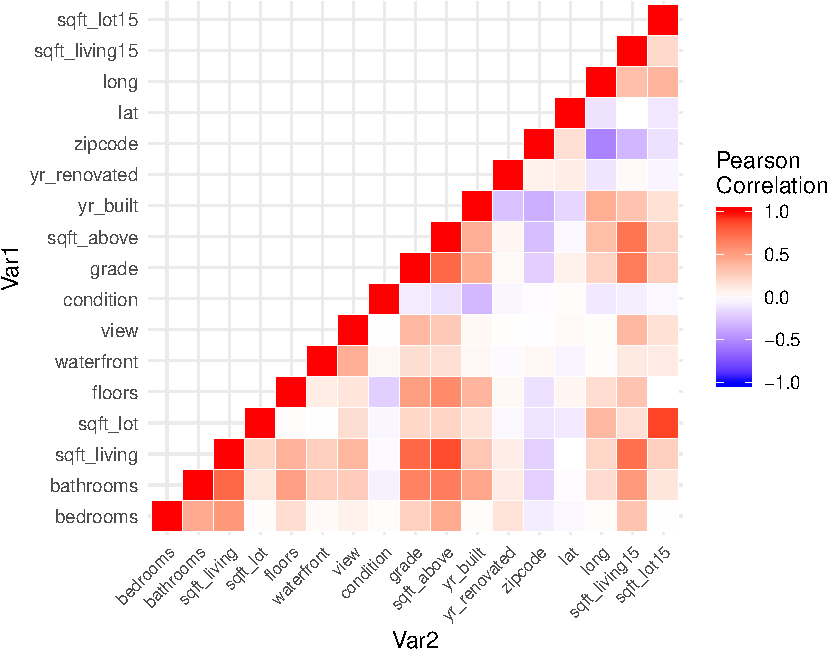
\includegraphics{FinalProjectForRegressionAnalysis_files/figure-latex/unnamed-chunk-8-1.pdf}






%
%==================================================================================================


\section{案例分析}




%
%--------------------------------------------------------------------------------------------------
\subsection{回归诊断}

\subsubsection{模型的诊断}

首先进行下面模型的拟合和诊断: \[
Price = X\beta  + \varepsilon
\]

其中,\(\beta\)包括了上述提到的18个特征。

\begin{Shaded}
\begin{Highlighting}[]
\NormalTok{lm.sol <-}\StringTok{ }\KeywordTok{lm}\NormalTok{(price}\OperatorTok{~}\NormalTok{., }\DataTypeTok{data =}\NormalTok{ data.trans)}
\KeywordTok{summary}\NormalTok{(lm.sol)}
\end{Highlighting}
\end{Shaded}

\begin{verbatim}
## Call:
## lm(formula = price ~ ., data = data.trans)

## Residuals:
##     Min      1Q  Median      3Q     Max 
## -400467  -78374  -10380   62692  745889 
## 
## Coefficients:
##                 Estimate Std. Error t value Pr(>|t|)    
## (Intercept)   -3.648e+06  2.187e+07  -0.167  0.86768    
## bedrooms      -3.528e+04  1.349e+04  -2.615  0.00968 ** 
## bathrooms      3.202e+04  2.547e+04   1.257  0.21044    
## sqft_living    1.100e+02  3.235e+01   3.399  0.00083 ***
## sqft_lot      -1.165e+00  5.300e-01  -2.199  0.02916 *  
## floors         6.905e+04  2.815e+04   2.453  0.01509 *  
## waterfront     1.892e+05  1.265e+05   1.496  0.13644    
## view           6.977e+04  1.494e+04   4.670 5.83e-06 ***
## condition      9.604e+03  1.717e+04   0.560  0.57649    
## grade          8.160e+04  1.732e+04   4.713 4.84e-06 ***
## sqft_above     2.395e+01  3.526e+01   0.679  0.49786    
## yr_built      -3.474e+03  5.439e+02  -6.387 1.38e-09 ***
## yr_renovated  -6.436e+00  2.841e+01  -0.227  0.82102    
## zipcode       -2.787e+02  2.511e+02  -1.110  0.26850    
## lat            5.234e+05  8.952e+04   5.847 2.27e-08 ***
## long          -1.008e+05  1.054e+05  -0.956  0.34035    
## sqft_living15  6.516e+01  2.781e+01   2.343  0.02022 *  
## sqft_lot15     1.543e+00  1.103e+00   1.399  0.16358    
## ---
## Signif. codes:  0 '***' 0.001 '**' 0.01 '*' 0.05 '.' 0.1 ' ' 1
## 
## Residual standard error: 148400 on 182 degrees of freedom
## Multiple R-squared:  0.7998, Adjusted R-squared:  0.7812 
## F-statistic: 42.78 on 17 and 182 DF,  p-value: < 2.2e-16
\end{verbatim}

\begin{Shaded}
\begin{Highlighting}[]
\KeywordTok{plot}\NormalTok{(lm.sol, }\DataTypeTok{which =} \DecValTok{1}\NormalTok{)}
\end{Highlighting}
\end{Shaded}

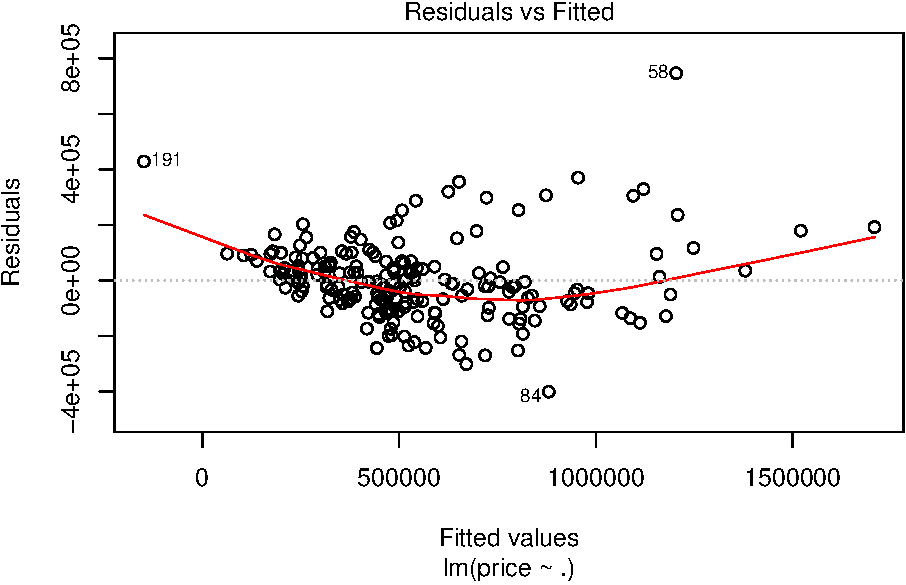
\includegraphics{FinalProjectForRegressionAnalysis_files/figure-latex/unnamed-chunk-9-1.pdf}

从残差图看出,这是一个喇叭型残差图,是方差齐性不符合的一个症状。
我们考虑对因变量\(price\)作变换,尝试\(z = log(y)\),得到回归方程 \[
z = X\beta +\varepsilon
\]

\begin{Shaded}
\begin{Highlighting}[]
\NormalTok{z <-}\StringTok{ }\KeywordTok{log}\NormalTok{(data.trans[, }\StringTok{'price'}\NormalTok{])}
\NormalTok{data2.trans <-}\StringTok{ }\KeywordTok{data.frame}\NormalTok{(z, data.trans[, }\OperatorTok{-}\StringTok{ }\DecValTok{1}\NormalTok{])}
\NormalTok{lm.sol2 <-}\StringTok{ }\KeywordTok{lm}\NormalTok{(z}\OperatorTok{~}\NormalTok{., }\DataTypeTok{data =}\NormalTok{ data2.trans)}
\KeywordTok{summary}\NormalTok{(lm.sol2)}
\end{Highlighting}
\end{Shaded}

\begin{verbatim}
## Call:
## lm(formula = z ~ ., data = data2.trans)
## 
## Residuals:
##      Min       1Q   Median       3Q      Max 
## -0.67735 -0.11967  0.00482  0.11253  0.58352 
## 
## Coefficients:
##                 Estimate Std. Error t value Pr(>|t|)    
## (Intercept)   -5.375e+01  3.430e+01  -1.567  0.11892    
## bedrooms      -4.460e-02  2.117e-02  -2.107  0.03647 *  
## bathrooms      7.378e-02  3.997e-02   1.846  0.06650 .  
## sqft_living    1.193e-04  5.076e-05   2.351  0.01981 *  
## sqft_lot      -1.419e-06  8.315e-07  -1.706  0.08969 .  
## floors         9.215e-02  4.416e-02   2.087  0.03830 *  
## waterfront     3.624e-01  1.984e-01   1.827  0.06940 .  
## view           7.196e-02  2.344e-02   3.070  0.00247 ** 
## condition      2.522e-02  2.693e-02   0.936  0.35027    
## grade          1.264e-01  2.717e-02   4.653 6.28e-06 ***
## sqft_above     5.839e-05  5.533e-05   1.055  0.29262    
## yr_built      -4.237e-03  8.534e-04  -4.965 1.57e-06 ***
## yr_renovated   1.934e-05  4.457e-05   0.434  0.66492    
## zipcode        4.965e-05  3.940e-04   0.126  0.89986    
## lat            1.356e+00  1.404e-01   9.654  < 2e-16 ***
## long          -3.224e-02  1.654e-01  -0.195  0.84566    
## sqft_living15  1.214e-04  4.363e-05   2.781  0.00599 ** 
## sqft_lot15     2.734e-06  1.731e-06   1.580  0.11589    
## ---
## Signif. codes:  0 '***' 0.001 '**' 0.01 '*' 0.05 '.' 0.1 ' ' 1
## 
## Residual standard error: 0.2328 on 182 degrees of freedom
## Multiple R-squared:  0.806,  Adjusted R-squared:  0.7879 
## F-statistic: 44.48 on 17 and 182 DF,  p-value: < 2.2e-16
\end{verbatim}

\begin{Shaded}
\begin{Highlighting}[]
\KeywordTok{plot}\NormalTok{(lm.sol2, }\DataTypeTok{which =} \DecValTok{1}\NormalTok{)}
\end{Highlighting}
\end{Shaded}

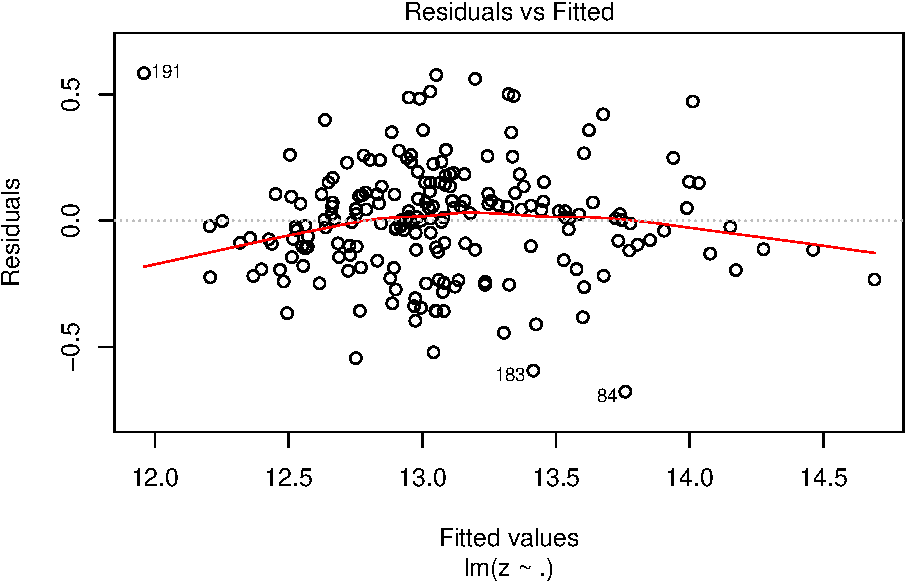
\includegraphics{FinalProjectForRegressionAnalysis_files/figure-latex/unnamed-chunk-10-1.pdf}

新的残差图不呈现任何明显的规则性,这表明我们的变化是合适的。

\begin{Shaded}
\begin{Highlighting}[]
\KeywordTok{plot}\NormalTok{(lm.sol2, }\DataTypeTok{which =} \DecValTok{2}\NormalTok{)}
\end{Highlighting}
\end{Shaded}

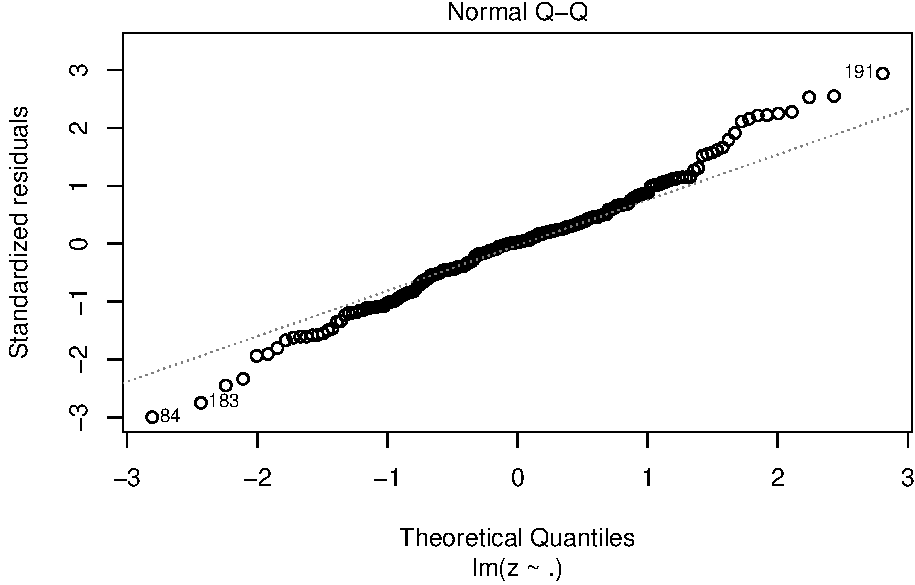
\includegraphics{FinalProjectForRegressionAnalysis_files/figure-latex/unnamed-chunk-11-1.pdf}

通过残差图和QQ图,我们接受线性假设、方差齐性假设、不相关性假设和正态性假设。

\subsubsection{数据的诊断}

\paragraph{异常点诊断}

\begin{Shaded}
\begin{Highlighting}[]
\NormalTok{y.fit <-}\StringTok{ }\KeywordTok{predict}\NormalTok{(lm.sol2)}
\NormalTok{e.std <-}\StringTok{ }\KeywordTok{rstandard}\NormalTok{(lm.sol2)}

\KeywordTok{plot}\NormalTok{(e.std}\OperatorTok{~}\NormalTok{y.fit)}
\KeywordTok{text}\NormalTok{(y.fit, e.std)}
\end{Highlighting}
\end{Shaded}

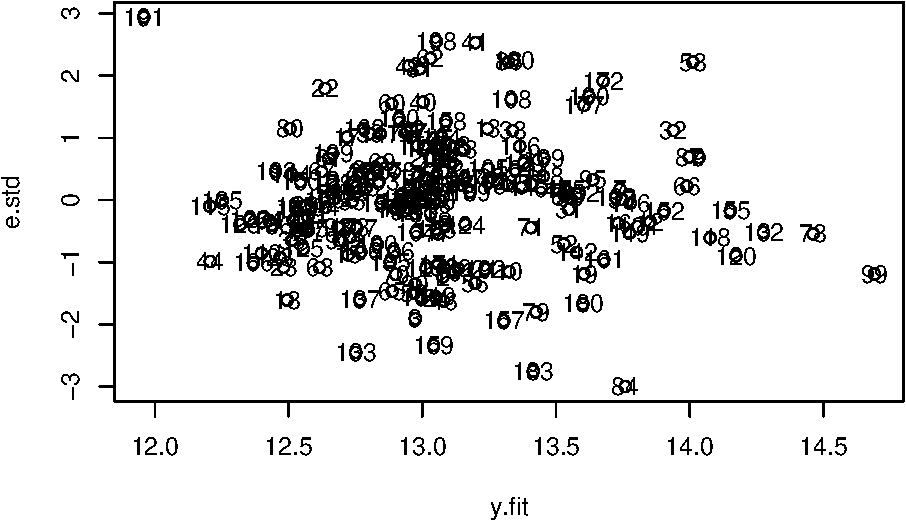
\includegraphics{FinalProjectForRegressionAnalysis_files/figure-latex/unnamed-chunk-13-1.pdf}
可以看到,其中有着许多数据的学生化残差是大于2的,我们将其打印出来。

\begin{Shaded}
\begin{Highlighting}[]
\NormalTok{point.abnormal <-}\StringTok{ }\KeywordTok{abs}\NormalTok{(e.std) }\OperatorTok{>}\StringTok{ }\DecValTok{2}
\NormalTok{point.abnormal <-}\StringTok{ }\NormalTok{(}\DecValTok{1}\OperatorTok{:}\DecValTok{200}\NormalTok{)[point.abnormal]}
\NormalTok{point.abnormal}
\end{Highlighting}
\end{Shaded}

\begin{verbatim}
##  [1]  41  42  58  62  81  84  86 100 133 159 183 191 198
\end{verbatim}

我们剔除学生化残差\(|r_i| > 2\)的异常点数据。

\begin{Shaded}
\begin{Highlighting}[]
\NormalTok{data2.trans <-}\StringTok{ }\NormalTok{data2.trans[}\OperatorTok{-}\KeywordTok{c}\NormalTok{(point.abnormal),]}
\end{Highlighting}
\end{Shaded}

\paragraph{强影响点诊断}

综合cook距离,我们将\(D_i > 0.01\)的数据,作为强影响点,将其打印出来如下。

\begin{Shaded}
\begin{Highlighting}[]
\NormalTok{influ.mea <-}\StringTok{ }\KeywordTok{influence.measures}\NormalTok{(lm.sol2)}
\NormalTok{point.influ <-}\StringTok{ }\NormalTok{influ.mea}\OperatorTok{$}\NormalTok{infmat[, }\StringTok{'cook.d'}\NormalTok{] }\OperatorTok{>}\StringTok{ }\FloatTok{0.01}
\NormalTok{point.influ <-}\StringTok{ }\NormalTok{(}\DecValTok{1}\OperatorTok{:}\DecValTok{200}\NormalTok{)[point.influ]}
\NormalTok{point.influ}
\end{Highlighting}
\end{Shaded}

\begin{verbatim}
##  [1]   3  22  28  41  42  46  56  58  62  65  84  86  89  99 100 101 108
## [18] 113 130 133 137 159 160 172 177 183 191 197 198
\end{verbatim}

\subsubsection{多重共线性诊断}

下面我们做多重共线性诊断。

\begin{Shaded}
\begin{Highlighting}[]
\CommentTok{# VIF}
\KeywordTok{vif}\NormalTok{(lm.sol2)}
\end{Highlighting}
\end{Shaded}

\begin{verbatim}
##      bedrooms     bathrooms   sqft_living      sqft_lot        floors 
##        1.8006        3.2566        7.2363        3.5865        2.1318 
##    waterfront          view     condition         grade    sqft_above 
##        1.4381        1.6057        1.3285        4.1328        7.1292 
##      yr_built  yr_renovated       zipcode           lat          long 
##        2.4939        1.2627        1.7185        1.1966        2.3457 
## sqft_living15    sqft_lot15 
##        3.1510        3.9131
\end{verbatim}

可以看到没有任何一个变量的VIF值大于10,因此不存在着多重共线性。

\begin{Shaded}
\begin{Highlighting}[]
\CommentTok{# 特征根诊断法}
\NormalTok{rho <-}\StringTok{ }\KeywordTok{cor}\NormalTok{(data.trans[, }\OperatorTok{-}\DecValTok{1}\NormalTok{])}
\KeywordTok{eigen}\NormalTok{(rho)}\OperatorTok{$}\NormalTok{values}
\end{Highlighting}
\end{Shaded}

\begin{verbatim}
##  [1] 5.28417978 2.14009690 1.59152696 1.37595250 1.19937212 1.08767712
##  [7] 0.84101974 0.72555094 0.55451358 0.51223902 0.48431923 0.34120744
## [13] 0.26190073 0.21565551 0.17827100 0.12830668 0.07821076
\end{verbatim}

再看特征根诊断法,其中没有特征根近似为零,则有不存在多重共线性关系。

\begin{Shaded}
\begin{Highlighting}[]
\CommentTok{# 条件数诊断法}
\KeywordTok{kappa}\NormalTok{(rho, }\DataTypeTok{exact =} \OtherTok{TRUE}\NormalTok{)}
\end{Highlighting}
\end{Shaded}

\begin{verbatim}
## [1] 67.56333
\end{verbatim}

最后看条件数诊断法,CI小于100,则可以认为没有多重共线性。

\begin{itemize}
\tightlist
\item
  结论:数据集不存在多重共线性。
\end{itemize}






%
%--------------------------------------------------------------------------------------------------
\subsection{线性回归}

\subsubsection{线性回归}\label{-1}

我们将回归诊断后的模型和数据标准化,重新运行一次模型。

\begin{Shaded}
\begin{Highlighting}[]
\NormalTok{data2.trans.scale <-}\StringTok{ }\KeywordTok{scale}\NormalTok{(data2.trans)}
\NormalTok{data3.trans <-}\StringTok{ }\KeywordTok{data.frame}\NormalTok{(data2.trans.scale)}
\NormalTok{lm.sol3 <-}\StringTok{ }\KeywordTok{lm}\NormalTok{(z}\OperatorTok{~}\NormalTok{., }\DataTypeTok{data =}\NormalTok{ data3.trans)}
\KeywordTok{summary}\NormalTok{(lm.sol3)}
\end{Highlighting}
\end{Shaded}

\begin{verbatim}
## Call:
## lm(formula = z ~ ., data = data3.trans)
## 
## Residuals:
##      Min       1Q   Median       3Q      Max 
## -0.79926 -0.23477  0.03316  0.25577  0.85355 
## 
## Coefficients:
##                 Estimate Std. Error t value Pr(>|t|)    
## (Intercept)   -1.365e-15  2.721e-02   0.000  1.00000    
## bedrooms      -6.160e-02  3.736e-02  -1.649  0.10106    
## bathrooms      5.789e-02  4.923e-02   1.176  0.24129    
## sqft_living    1.940e-01  7.656e-02   2.534  0.01219 *  
## sqft_lot      -9.258e-02  5.247e-02  -1.765  0.07944 .  
## floors         1.320e-01  4.040e-02   3.268  0.00131 ** 
## waterfront     9.810e-02  3.323e-02   2.952  0.00360 ** 
## view           8.710e-02  3.521e-02   2.474  0.01437 *  
## condition      7.812e-02  3.228e-02   2.420  0.01657 *  
## grade          3.541e-01  5.728e-02   6.182 4.59e-09 ***
## sqft_above     4.176e-02  7.572e-02   0.552  0.58202    
## yr_built      -2.275e-01  4.306e-02  -5.283 3.87e-07 ***
## yr_renovated   6.237e-02  3.104e-02   2.009  0.04613 *  
## zipcode        6.622e-02  3.636e-02   1.821  0.07036 .  
## lat            3.445e-01  2.997e-02  11.495  < 2e-16 ***
## long          -1.085e-02  4.223e-02  -0.257  0.79755    
## sqft_living15  2.476e-01  4.927e-02   5.027 1.26e-06 ***
## sqft_lot15     1.059e-01  5.451e-02   1.943  0.05364 .  
## ---
## Signif. codes:  0 '***' 0.001 '**' 0.01 '*' 0.05 '.' 0.1 ' ' 1
## 
## Residual standard error: 0.3721 on 169 degrees of freedom
## Multiple R-squared:  0.8742, Adjusted R-squared:  0.8616 
## F-statistic: 69.09 on 17 and 169 DF,  p-value: < 2.2e-16
\end{verbatim}

\begin{Shaded}
\begin{Highlighting}[]
\KeywordTok{plot}\NormalTok{(lm.sol3, }\DataTypeTok{which =} \DecValTok{1}\NormalTok{)}
\end{Highlighting}
\end{Shaded}

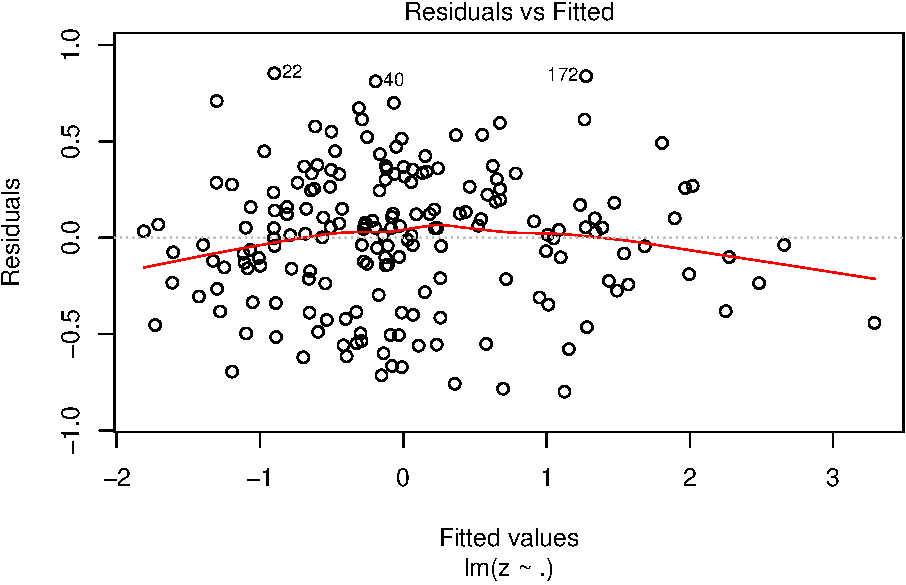
\includegraphics{FinalProjectForRegressionAnalysis_files/figure-latex/unnamed-chunk-21-1.pdf}

\paragraph{\texorpdfstring{对回归方程的显著性作检验(显著性水平\(\alpha = 0.05\))}{对回归方程的显著性作检验(显著性水平\textbackslash{}alpha = 0.05)}}\label{alpha-0.05}

可以看到,\(F_H = 69.09\), p值小于\(2.2\times 10 ^{-6} < 0.05\),
所以我们认为回归自变量对因变量有着显著的线性影响。

\paragraph{\texorpdfstring{对每一个回归系数的显著性作检验(显著性水平\(\alpha = 0.05\))}{对每一个回归系数的显著性作检验(显著性水平\textbackslash{}alpha = 0.05)}}\label{alpha-0.05}

可以看到,bedrooms、bathrooms、sqft\_lot、sqft\_above、zipcode、long、sqft\_lot15的p值均大于0.05,我们接受对应自变量的显著性假设。因此我们需要进行变量选择。

\subsubsection{变量选择}

\paragraph{自变量选择的准则}

首先对所有子模型进行运行,得到所有子模型的各个准则,总共有131071个子模型。
\begin{verbatim}
## [1] "The number of submodel"
## [1] 131071
\end{verbatim}


\begin{Shaded}
\begin{Highlighting}[]
\NormalTok{formu <-}\StringTok{ }\KeywordTok{paste}\NormalTok{(yname, }\StringTok{"~."}\NormalTok{)}
\NormalTok{search.results <-}\StringTok{ }\KeywordTok{regsubsets}\NormalTok{(}\KeywordTok{as.formula}\NormalTok{(formu), }\DataTypeTok{data =}\NormalTok{ data3.trans,}
                             \DataTypeTok{method =} \StringTok{"exhaustive"}\NormalTok{, }\DataTypeTok{nbest =}\NormalTok{ nbest,}
                             \DataTypeTok{really.big =}\NormalTok{ T)}
\NormalTok{selection.criteria <-}\StringTok{ }\KeywordTok{summary}\NormalTok{(search.results)}

\NormalTok{n <-}\StringTok{ }\KeywordTok{length}\NormalTok{(data3.trans[, }\DecValTok{1}\NormalTok{])}
\NormalTok{q <-}\StringTok{ }\KeywordTok{as.integer}\NormalTok{(}\KeywordTok{row.names}\NormalTok{(selection.criteria}\OperatorTok{$}\NormalTok{which))}
\NormalTok{R.sq <-}\StringTok{ }\NormalTok{selection.criteria}\OperatorTok{$}\NormalTok{rsq}
\NormalTok{AdjR.sq <-}\StringTok{ }\NormalTok{selection.criteria}\OperatorTok{$}\NormalTok{adjr2}
\NormalTok{rms <-}\StringTok{ }\NormalTok{selection.criteria}\OperatorTok{$}\NormalTok{rss }\OperatorTok{/}\StringTok{ }\NormalTok{(n }\OperatorTok{-}\StringTok{ }\NormalTok{q }\OperatorTok{-}\StringTok{ }\DecValTok{1}\NormalTok{)}
\NormalTok{Cp <-}\StringTok{ }\NormalTok{selection.criteria}\OperatorTok{$}\NormalTok{cp}
\NormalTok{aic.f <-}\StringTok{ }\NormalTok{n }\OperatorTok{*}\StringTok{ }\KeywordTok{log}\NormalTok{(selection.criteria}\OperatorTok{$}\NormalTok{rss) }\OperatorTok{+}\StringTok{ }\DecValTok{2} \OperatorTok{*}\StringTok{ }\NormalTok{(q }\OperatorTok{+}\StringTok{ }\DecValTok{1}\NormalTok{)}
\NormalTok{bic.f <-}\StringTok{ }\NormalTok{n }\OperatorTok{*}\StringTok{ }\KeywordTok{log}\NormalTok{(selection.criteria}\OperatorTok{$}\NormalTok{rss) }\OperatorTok{+}\StringTok{ }\NormalTok{(q }\OperatorTok{+}\StringTok{ }\DecValTok{1}\NormalTok{) }\OperatorTok{*}\StringTok{ }\KeywordTok{log}\NormalTok{(n)}
\NormalTok{var <-}\StringTok{ }\KeywordTok{as.matrix}\NormalTok{(selection.criteria}\OperatorTok{$}\NormalTok{which[, }\DecValTok{2}\OperatorTok{:}\StringTok{ }\KeywordTok{length}\NormalTok{(data3.trans[}\DecValTok{1}\NormalTok{,]) ])}
\NormalTok{press.f <-}\StringTok{ }\KeywordTok{calcuPress}\NormalTok{(data3.trans, var, nbest, }\DataTypeTok{yname =}\NormalTok{ yname)}
\NormalTok{criteria.table <-}\StringTok{ }\KeywordTok{data.frame}\NormalTok{(}\KeywordTok{cbind}\NormalTok{(q, rms, R.sq, AdjR.sq, Cp, aic.f, bic.f, press.f), var)}
\end{Highlighting}
\end{Shaded}

\begin{itemize}
\tightlist
\item
  调整后的\(R^2\)准则
  可以得到,根据调整后的\(R^2\)准则,我们选择以下自变量子集:
\end{itemize}

\begin{Shaded}
\begin{Highlighting}[]
\NormalTok{var.AdjR.sq <-}\StringTok{ }\NormalTok{criteria.table[}\KeywordTok{which.max}\NormalTok{(criteria.table[,}\StringTok{'AdjR.sq'}\NormalTok{]), ]}
\NormalTok{varnameList[}\KeywordTok{as.matrix}\NormalTok{(var.AdjR.sq[}\DecValTok{1}\NormalTok{, }\DecValTok{9}\OperatorTok{:}\DecValTok{25}\NormalTok{])[}\DecValTok{1}\NormalTok{, ]]}
\end{Highlighting}
\end{Shaded}

\begin{verbatim}
## [1] "sqft_living"   "floors"        "waterfront"    "view"         
## [5] "grade"         "yr_built"      "lat"           "sqft_living15"
\end{verbatim}

\begin{itemize}
\tightlist
\item
  \(Cp\)准则 可以得到,根据\(Cp\)准则,我们选择以下自变量子集:
\end{itemize}

\begin{Shaded}
\begin{Highlighting}[]
\NormalTok{var.Cp <-}\StringTok{ }\NormalTok{criteria.table[}\KeywordTok{which.min}\NormalTok{(criteria.table[,}\StringTok{'Cp'}\NormalTok{]),]}
\NormalTok{varnameList[}\KeywordTok{as.matrix}\NormalTok{(var.Cp[}\DecValTok{1}\NormalTok{, }\DecValTok{9}\OperatorTok{:}\DecValTok{25}\NormalTok{])[}\DecValTok{1}\NormalTok{, ]]}
\end{Highlighting}
\end{Shaded}

\begin{verbatim}
## [1] "sqft_living"   "floors"        "waterfront"    "view"         
## [5] "grade"         "yr_built"      "lat"           "sqft_living15"
\end{verbatim}

\begin{itemize}
\tightlist
\item
  \(AIC\)准则 可以得到,根据\(AIC\)准则,我们选择以下自变量子集:
\end{itemize}

\begin{Shaded}
\begin{Highlighting}[]
\NormalTok{var.aic.f <-}\StringTok{ }\NormalTok{criteria.table[}\KeywordTok{which.min}\NormalTok{(criteria.table[,}\StringTok{'aic.f'}\NormalTok{]),]}
\NormalTok{varnameList[}\KeywordTok{as.matrix}\NormalTok{(var.aic.f[}\DecValTok{1}\NormalTok{, }\DecValTok{9}\OperatorTok{:}\DecValTok{25}\NormalTok{])[}\DecValTok{1}\NormalTok{, ]]}
\end{Highlighting}
\end{Shaded}

\begin{verbatim}
## [1] "sqft_living"   "floors"        "waterfront"    "view"         
## [5] "grade"         "yr_built"      "lat"           "sqft_living15"
\end{verbatim}

\begin{itemize}
\tightlist
\item
  \(BIC\)准则 可以得到,根据\(BIC\)准则,我们同样选择以下自变量子集:
\end{itemize}

\begin{Shaded}
\begin{Highlighting}[]
\NormalTok{var.bic.f<-}\StringTok{ }\NormalTok{criteria.table[}\KeywordTok{which.min}\NormalTok{(criteria.table[,}\StringTok{'bic.f'}\NormalTok{]),]}
\NormalTok{varnameList[}\KeywordTok{as.matrix}\NormalTok{(var.bic.f[}\DecValTok{1}\NormalTok{, }\DecValTok{9}\OperatorTok{:}\DecValTok{25}\NormalTok{])[}\DecValTok{1}\NormalTok{, ]]}
\end{Highlighting}
\end{Shaded}

\begin{verbatim}
## [1] "sqft_living"   "floors"        "waterfront"    "grade"        
## [5] "yr_built"      "lat"           "sqft_living15"
\end{verbatim}

\begin{itemize}
\tightlist
\item
  \(PRESS\)准则
  可以得到,根据\(PRESS\)准则,我们同样选择以下自变量子集:
\end{itemize}

\begin{Shaded}
\begin{Highlighting}[]
\NormalTok{var.press.f <-}\StringTok{ }\NormalTok{criteria.table[}\KeywordTok{which.min}\NormalTok{(criteria.table[,}\StringTok{'press.f'}\NormalTok{]),]}
\NormalTok{varnameList[}\KeywordTok{as.matrix}\NormalTok{(var.press.f[}\DecValTok{1}\NormalTok{, }\DecValTok{9}\OperatorTok{:}\DecValTok{25}\NormalTok{])[}\DecValTok{1}\NormalTok{, ]]}
\end{Highlighting}
\end{Shaded}

\begin{verbatim}
## [1] "sqft_living"   "floors"        "waterfront"    "view"         
## [5] "grade"         "yr_built"      "lat"           "sqft_living15"
\end{verbatim}

\paragraph{逐步回归法}

我们使用\(SignifReg\)函数进行逐步回归,这个函数相比于\(step\)函数有三个优点:

\begin{itemize}
\tightlist
\item
  具有更多的criterion。除了\(step\)函数有的\(AIC\)准则外,还具有\(BIC\)、\(C_p\)、\(r-adj\)、\(p-value\)等准则。
\item
  在模型选择过程中,会同步进行变量回归系数的显著性检验。如若没有通过\(\alpha\)置信水平的检验,则不将变量选入模型中。
\item
  此外,对于逐步回归法,除了从一个空模型开始之外,还能够从一个全模型开始,逐步删除变量。
\end{itemize}

\begin{Shaded}
\begin{Highlighting}[]
\NormalTok{yname <-}\StringTok{ "z"}
\NormalTok{varnameList <-}\StringTok{ }\KeywordTok{colnames}\NormalTok{(data3.trans)}
\NormalTok{varnameList <-}\StringTok{ }\NormalTok{varnameList[}\OperatorTok{-}\StringTok{ }\KeywordTok{which}\NormalTok{(varnameList }\OperatorTok{==}\StringTok{ }\NormalTok{yname)]}
\NormalTok{formu <-}\StringTok{ }\KeywordTok{as.formula}\NormalTok{(}\KeywordTok{paste}\NormalTok{(yname, }\KeywordTok{paste}\NormalTok{(}\StringTok{"~"}\NormalTok{, }\KeywordTok{paste}\NormalTok{(varnameList, }\DataTypeTok{collapse =} \StringTok{"+"}\NormalTok{))))}
\NormalTok{step.model <-}\StringTok{ }\KeywordTok{SignifReg}\NormalTok{(}\DataTypeTok{scope =}\NormalTok{ formu, }\DataTypeTok{data =}\NormalTok{ data3.trans, }\DataTypeTok{alpha =} \FloatTok{0.05}\NormalTok{, }
                        \DataTypeTok{direction =} \StringTok{"step_null"}\NormalTok{, }\DataTypeTok{criterion =} \StringTok{"AIC"}\NormalTok{)}
\end{Highlighting}
\end{Shaded}

\begin{verbatim}
## Call:
## lm(formula = formu, data = data3.trans)
## 
## Residuals:
##      Min       1Q   Median       3Q      Max 
## -0.92360 -0.23559  0.00277  0.27197  0.85419 
## 
## Coefficients:
##                 Estimate Std. Error t value Pr(>|t|)    
## (Intercept)   -5.816e-15  2.816e-02   0.000 1.000000    
## grade          4.179e-01  5.171e-02   8.082 9.20e-14 ***
## lat            3.533e-01  2.969e-02  11.900  < 2e-16 ***
## sqft_living    2.242e-01  4.941e-02   4.537 1.04e-05 ***
## yr_built      -2.776e-01  3.353e-02  -8.280 2.78e-14 ***
## waterfront     1.641e-01  2.873e-02   5.713 4.56e-08 ***
## sqft_living15  2.460e-01  4.653e-02   5.287 3.59e-07 ***
## floors         1.193e-01  3.489e-02   3.420 0.000777 ***
## ---
## Signif. codes:  0 '***' 0.001 '**' 0.01 '*' 0.05 '.' 0.1 ' ' 1
## 
## Residual standard error: 0.385 on 179 degrees of freedom
## Multiple R-squared:  0.8573, Adjusted R-squared:  0.8517 
## F-statistic: 153.6 on 7 and 179 DF,  p-value: < 2.2e-16
\end{verbatim}

可以看到,逐步回归法得到的结果,选取了grade, lat, sqft\_living,
yr\_built, waterfront, sqft\_living15,
floors共7个自变量。得到的回归方程为:
\begin{align*}
z^* = & 0.4179\ grade^* + 0.3533\ lat^* + 0.2242\ sqft\_living ^* \\
& + -0.2776\ yr\_built^* + 0.1641\ waterfront^* + 0.246\ sqft\_living15^* \\
& + 0.1193\ floors^*
\end{align*}
上述方程是经过标准化后的,我们将其还原成原来的系数,如下:
\begin{align*}
z = & 4.5396\ grade + 35.7958\ lat + 0.0033\ sqft\_living \\
& + -0.1177\ yr\_built + 20.7789\ waterfront + 0.0047 sqft\_living15 \\
& + 2.8302\ floors -1513.858
\end{align*}
即:
\begin{align*}
\log{(y)} = & 4.5396\ grade + 35.7958\ lat + 0.0033\ sqft\_living \\
& + -0.1177\ yr\_built + 20.7789\ waterfront + 0.0047 sqft\_living15 \\
& + 2.8302\ floors -1513.858
\end{align*}






%
%--------------------------------------------------------------------------------------------------
\subsection{主成分回归}

由于上述线性回归过程中,我们可以看到自变量个数较多,下面尝试主成分回归方法。

\begin{Shaded}
\begin{Highlighting}[]
\NormalTok{yname <-}\StringTok{ "z"}
\NormalTok{varnameList <-}\StringTok{ }\KeywordTok{colnames}\NormalTok{(data3.trans)}
\NormalTok{varnameList <-}\StringTok{ }\NormalTok{varnameList[}\OperatorTok{-}\StringTok{ }\KeywordTok{which}\NormalTok{(varnameList }\OperatorTok{==}\StringTok{ }\NormalTok{yname)]}
\NormalTok{formu <-}\StringTok{ }\KeywordTok{as.formula}\NormalTok{(}\KeywordTok{paste}\NormalTok{(}\StringTok{"~"}\NormalTok{, }\KeywordTok{paste}\NormalTok{(varnameList, }\DataTypeTok{collapse =} \StringTok{"+"}\NormalTok{)))}
\NormalTok{y.pr <-}\StringTok{ }\KeywordTok{princomp}\NormalTok{(formu, }\DataTypeTok{data =}\NormalTok{ data3.trans, }\DataTypeTok{cor =} \OtherTok{TRUE}\NormalTok{)}
\KeywordTok{summary}\NormalTok{(y.pr)}
\end{Highlighting}
\end{Shaded}

\begin{verbatim}
## Importance of components:
##                           Comp.1    Comp.2     Comp.3     Comp.4
## Standard deviation     2.3270123 1.4407455 1.26992673 1.18082869
## Proportion of Variance 0.3185286 0.1221028 0.09486552 0.08202096
## Cumulative Proportion  0.3185286 0.4406314 0.53549692 0.61751788
##                            Comp.5     Comp.6     Comp.7     Comp.8
## Standard deviation     1.08988417 1.05454190 0.92136091 0.83712864
## Proportion of Variance 0.06987338 0.06541521 0.04993564 0.04122261
## Cumulative Proportion  0.68739127 0.75280648 0.80274212 0.84396473
##                            Comp.9    Comp.10    Comp.11    Comp.12
## Standard deviation     0.72533956 0.71395682 0.67055480 0.56875075
## Proportion of Variance 0.03094809 0.02998437 0.02644963 0.01902808
## Cumulative Proportion  0.87491282 0.90489719 0.93134682 0.95037491
##                           Comp.13    Comp.14    Comp.15     Comp.16
## Standard deviation     0.51029847 0.46281328 0.42236338 0.344631100
## Proportion of Variance 0.01531791 0.01259977 0.01049358 0.006986506
## Cumulative Proportion  0.96569282 0.97829259 0.98878617 0.995772675
##                            Comp.17
## Standard deviation     0.268075585
## Proportion of Variance 0.004227325
## Cumulative Proportion  1.000000000
\end{verbatim}

可以看到,前9个主成分的Cumulative
Proportion达到了0.87491282,我们可以只选取前9个主成分,删除后8个主成分。

前九个主成分对应的标准正交化特征向量可由下面这个命令打印出来。我们只查看前4个标准正交化特征向量。

\begin{Shaded}
\begin{Highlighting}[]
\NormalTok{y.pr}\OperatorTok{$}\NormalTok{loadings[, }\DecValTok{1}\OperatorTok{:}\DecValTok{9}\NormalTok{]}
\end{Highlighting}
\end{Shaded}

\begin{verbatim}
##                    Comp.1      Comp.2       Comp.3      Comp.4
## bedrooms       0.17275752  0.26633220  0.020224937  0.50175944
## bathrooms      0.32210921  0.20370328 -0.031434934  0.02101727
## sqft_living    0.36722569  0.17906689 -0.132195885  0.18932991
## sqft_lot       0.15998719 -0.50084208 -0.199735800  0.13550622
## floors         0.26378636  0.21097062  0.072467151 -0.28804415
## waterfront     0.04533319 -0.04403962 -0.440505893 -0.25970622
## view           0.15940143 -0.05741524 -0.530455853 -0.12144031
## condition     -0.07877952 -0.04929760 -0.095049354  0.40840179
## grade          0.36418604  0.06917520 -0.105471467 -0.07991571
## sqft_above     0.38946624  0.12948326  0.026510238  0.03534522
## yr_built       0.26086170 -0.07965103  0.310507821 -0.37090949
## yr_renovated  -0.03979088  0.17871531 -0.114050930  0.38320617
## zipcode       -0.18645856  0.18665379 -0.422455385 -0.13786490
## lat           -0.02310463  0.24204175 -0.132707417 -0.18255780
## long           0.24069459 -0.35901771  0.285915449  0.05224916
## sqft_living15  0.35409497  0.06490277 -0.009420864  0.06036788
## sqft_lot15     0.17358343 -0.51587308 -0.228805553  0.10424251
\end{verbatim}

计算主成分得分,进行主成分估计:

\begin{Shaded}
\begin{Highlighting}[]
\NormalTok{pre =}\StringTok{ }\KeywordTok{predict}\NormalTok{(y.pr)}
\NormalTok{z <-}\StringTok{ }\NormalTok{data3.trans}\OperatorTok{$}\NormalTok{z}
\NormalTok{data3.trans.pc <-}\StringTok{ }\KeywordTok{data.frame}\NormalTok{(z, pre[, }\DecValTok{1}\OperatorTok{:}\DecValTok{9}\NormalTok{])}
\NormalTok{pc.sol <-}\StringTok{ }\KeywordTok{lm}\NormalTok{(z}\OperatorTok{~}\NormalTok{., }\DataTypeTok{data =}\NormalTok{ data3.trans.pc)}
\KeywordTok{summary}\NormalTok{(pc.sol)}
\end{Highlighting}
\end{Shaded}

\begin{verbatim}
## Call:
## lm(formula = z ~ ., data = data3.trans.pc)
## 
## Residuals:
##      Min       1Q   Median       3Q      Max 
## -0.83950 -0.24359 -0.00438  0.23949  1.12940 
## 
## Coefficients:
##               Estimate Std. Error t value Pr(>|t|)    
## (Intercept) -7.897e-16  2.818e-02   0.000 1.000000    
## Comp.1       2.773e-01  1.211e-02  22.898  < 2e-16 ***
## Comp.2       2.108e-01  1.956e-02  10.780  < 2e-16 ***
## Comp.3      -3.140e-01  2.219e-02 -14.152  < 2e-16 ***
## Comp.4      -1.279e-02  2.386e-02  -0.536 0.592515    
## Comp.5      -5.325e-02  2.585e-02  -2.060 0.040894 *  
## Comp.6      -3.369e-01  2.672e-02 -12.609  < 2e-16 ***
## Comp.7      -2.310e-01  3.058e-02  -7.555 2.16e-12 ***
## Comp.8      -5.166e-02  3.366e-02  -1.535 0.126611    
## Comp.9      -1.350e-01  3.885e-02  -3.476 0.000641 ***
## ---
## Signif. codes:  0 '***' 0.001 '**' 0.01 '*' 0.05 '.' 0.1 ' ' 1
## 
## Residual standard error: 0.3853 on 177 degrees of freedom
## Multiple R-squared:  0.8587, Adjusted R-squared:  0.8515 
## F-statistic: 119.5 on 9 and 177 DF,  p-value: < 2.2e-16
\end{verbatim}

可以看到,有第4、第8个主成分没有通过单变量回归系数的显著性检验,我们再次进行变量选择:

\begin{Shaded}
\begin{Highlighting}[]
\NormalTok{yname <-}\StringTok{ "z"}
\NormalTok{varnameList <-}\StringTok{ }\KeywordTok{colnames}\NormalTok{(data3.trans.pc)}
\NormalTok{varnameList <-}\StringTok{ }\NormalTok{varnameList[}\OperatorTok{-}\StringTok{ }\KeywordTok{which}\NormalTok{(varnameList }\OperatorTok{==}\StringTok{ }\NormalTok{yname)]}
\NormalTok{formu <-}\StringTok{ }\KeywordTok{as.formula}\NormalTok{(}\KeywordTok{paste}\NormalTok{(yname, }\KeywordTok{paste}\NormalTok{(}\StringTok{"~"}\NormalTok{, }\KeywordTok{paste}\NormalTok{(varnameList, }\DataTypeTok{collapse =} \StringTok{"+"}\NormalTok{))))}
\NormalTok{step.model.pc <-}\StringTok{ }\KeywordTok{SignifReg}\NormalTok{(}\DataTypeTok{scope =}\NormalTok{ formu, }\DataTypeTok{data =}\NormalTok{ data3.trans.pc, }\DataTypeTok{alpha =} \FloatTok{0.05}\NormalTok{, }
                           \DataTypeTok{direction =} \StringTok{"step_null"}\NormalTok{, }\DataTypeTok{criterion =} \StringTok{"r-adj"}\NormalTok{)}
\end{Highlighting}
\end{Shaded}

\begin{verbatim}
## Call:
## lm(formula = formu, data = data3.trans.pc)
## 
## Residuals:
##     Min      1Q  Median      3Q     Max 
## -1.0395 -0.2624  0.0287  0.2719  1.1312 
## 
## Coefficients:
##               Estimate Std. Error t value Pr(>|t|)    
## (Intercept) -7.949e-16  2.848e-02   0.000 1.000000    
## Comp.1       2.773e-01  1.224e-02  22.654  < 2e-16 ***
## Comp.3      -3.140e-01  2.243e-02 -14.001  < 2e-16 ***
## Comp.6      -3.369e-01  2.701e-02 -12.475  < 2e-16 ***
## Comp.2       2.108e-01  1.977e-02  10.666  < 2e-16 ***
## Comp.7      -2.310e-01  3.091e-02  -7.475 3.26e-12 ***
## Comp.9      -1.350e-01  3.926e-02  -3.439 0.000726 ***
## ---
## Signif. codes:  0 '***' 0.001 '**' 0.01 '*' 0.05 '.' 0.1 ' ' 1
## 
## Residual standard error: 0.3895 on 180 degrees of freedom
## Multiple R-squared:  0.8532, Adjusted R-squared:  0.8483 
## F-statistic: 174.4 on 6 and 180 DF,  p-value: < 2.2e-16
\end{verbatim}

最终,我们可以得到第1、2、3、6、7、9个主成分选入模型,它们的累计贡献值达到了0.6817959,回归模型如下:
\begin{align*}
z^* = & 0.2773\ Comp.1 + -0.314\ Comp.3 + -0.3369\ Comp.6 \\
& + 0.2108\ Comp.2 + -0.231\ Comp.7 + -0.135\ Comp.9
\end{align*}
也就是
\begin{align*}
z^* = & 1.7626\ bedrooms^* + 1.244\ bathrooms^* + 0.3888\ sqft\_living^* \\
& + 0.186\ sqft_lot^* + 0.9191\ floors^* -0.776\ waterfront^* \\
& -0.7024\ view^* -0.3198\ condition^* -0.2675\ grade^* \\
& + 0.3662\ sqft\_above^* + 0.71\ yr\_built^* + 0.5819\ yr\_renovated^* \\
& + 0.0634\ zipcode^* -0.9196\ lat^* -0.1973\ long^*  \\
& -0.3737\ sqft\_living15^* -0.2022\ sqft\_lot15^*
\end{align*}
即
\begin{align*}
\log{(y)} = & 21.9432\ bathrooms + 0.0057\ sqft\_living + 0.0001 sqft\_lot \\
& + 21.8017\ floors -98.241\ waterfront -10.4364\ view \\
& -5.9259\ condition -2.9055\ grade + 0.0059\ sqft\_above \\
& + 0.3011\ yr\_built + 0.0187\ yr\_renovated + 0.0151\ zipcode\\
& -93.1814\ lat -16.9743\ long -0.0072\ sqft\_living15 \\
& -0.0001\ sqft\_lot15 + 254.5485
\end{align*}







%
%--------------------------------------------------------------------------------------------------
\subsection{岭回归}

下面我们用岭估计的方法寻找岭回归方程。

\begin{Shaded}
\begin{Highlighting}[]
\NormalTok{yname <-}\StringTok{ "z"}
\NormalTok{varnameList <-}\StringTok{ }\KeywordTok{colnames}\NormalTok{(data3.trans)}
\NormalTok{varnameList <-}\StringTok{ }\NormalTok{varnameList[}\OperatorTok{-}\StringTok{ }\KeywordTok{which}\NormalTok{(varnameList }\OperatorTok{==}\StringTok{ }\NormalTok{yname)]}
\NormalTok{formu <-}\StringTok{ }\KeywordTok{as.formula}\NormalTok{(}\KeywordTok{paste}\NormalTok{(}\KeywordTok{paste}\NormalTok{(yname, }\StringTok{"~"}\NormalTok{), }\KeywordTok{paste}\NormalTok{(varnameList, }\DataTypeTok{collapse =} \StringTok{"+"}\NormalTok{)))}
\NormalTok{rr.sol <-}\StringTok{ }\KeywordTok{lm.ridge}\NormalTok{(formu, }\DataTypeTok{data =}\NormalTok{ data3.trans, }
                   \DataTypeTok{lambda =} \KeywordTok{c}\NormalTok{(}\KeywordTok{seq}\NormalTok{(}\DecValTok{0}\NormalTok{, }\DecValTok{1000}\NormalTok{, }\DataTypeTok{by =} \DecValTok{1}\NormalTok{)))}
\KeywordTok{plot}\NormalTok{(rr.sol)}
\end{Highlighting}
\end{Shaded}

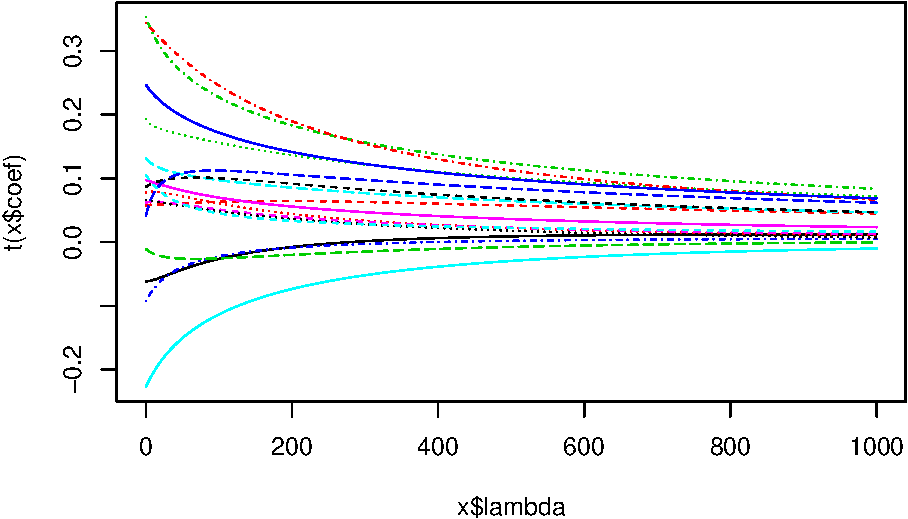
\includegraphics{FinalProjectForRegressionAnalysis_files/figure-latex/unnamed-chunk-33-1.pdf}

可以看到,岭回归的方法需要较大的\(\lambda\)才能够使得岭迹图趋于平稳。我们选取\(\lambda = 400\)进行分析。

\begin{Shaded}
\begin{Highlighting}[]
\NormalTok{yname <-}\StringTok{ "z"}
\NormalTok{varnameList <-}\StringTok{ }\KeywordTok{colnames}\NormalTok{(data3.trans)}
\NormalTok{varnameList <-}\StringTok{ }\NormalTok{varnameList[}\OperatorTok{-}\StringTok{ }\KeywordTok{which}\NormalTok{(varnameList }\OperatorTok{==}\StringTok{ }\NormalTok{yname)]}
\NormalTok{formu <-}\StringTok{ }\KeywordTok{as.formula}\NormalTok{(}\KeywordTok{paste}\NormalTok{(}\KeywordTok{paste}\NormalTok{(yname, }\StringTok{"~"}\NormalTok{), }\KeywordTok{paste}\NormalTok{(varnameList, }\DataTypeTok{collapse =} \StringTok{"+"}\NormalTok{)))}
\NormalTok{ridge.model <-}\StringTok{ }\KeywordTok{lm.ridge}\NormalTok{(formu, }\DataTypeTok{data =}\NormalTok{ data3.trans, }
                        \DataTypeTok{lambda =} \DecValTok{400}\NormalTok{)}
\NormalTok{ridge.model}
\end{Highlighting}
\end{Shaded}

\begin{verbatim}
##                    bedrooms     bathrooms   sqft_living      sqft_lot 
## -1.506414e-15  6.373284e-03  6.052329e-02  1.107143e-01  2.458317e-04 
##        floors    waterfront          view     condition         grade 
##  7.034580e-02  4.097970e-02  7.479548e-02  2.710777e-02  1.381468e-01 
##    sqft_above      yr_built  yr_renovated       zipcode           lat 
##  9.055236e-02 -3.863127e-02  2.649473e-02  2.225569e-02  1.304872e-01 
##          long sqft_living15    sqft_lot15 
## -1.068821e-02  1.095004e-01  2.481061e-02
\end{verbatim}









%
%--------------------------------------------------------------------------------------------------
\subsection{预测}

\subsubsection{测试集数据变换}

首先对测试集数据,做与训练集一样的scale变换。

\begin{Shaded}
\begin{Highlighting}[]
\NormalTok{data2.trans.scale.center <-}\StringTok{ }\KeywordTok{attr}\NormalTok{(data2.trans.scale,}\StringTok{"scaled:center"}\NormalTok{)}
\NormalTok{data2.trans.scale.scale <-}\StringTok{ }\KeywordTok{attr}\NormalTok{(data2.trans.scale,}\StringTok{"scaled:scale"}\NormalTok{)}
\NormalTok{data2.test <-}\StringTok{ }\NormalTok{data.test}
\ControlFlowTok{for}\NormalTok{ (i }\ControlFlowTok{in} \KeywordTok{colnames}\NormalTok{(data.test))\{}
\NormalTok{  data2.test[i] <-}\StringTok{ }\NormalTok{(data.test[i] }\OperatorTok{-}\StringTok{ }\NormalTok{data2.trans.scale.center[i]) }\OperatorTok{/}\StringTok{ }\NormalTok{data2.trans.scale.scale[i]}
\NormalTok{\}}
\NormalTok{data2.test <-}\StringTok{ }\NormalTok{data2.test[}\OperatorTok{-}\DecValTok{1}\NormalTok{]}

\NormalTok{y.test <-}\StringTok{ }\NormalTok{data.test}\OperatorTok{$}\NormalTok{price}
\NormalTok{y.center <-}\StringTok{ }\NormalTok{data2.trans.scale.center[}\StringTok{"z"}\NormalTok{]}
\NormalTok{y.scale <-}\StringTok{ }\NormalTok{data2.trans.scale.scale[}\StringTok{"z"}\NormalTok{]}
\NormalTok{y.log.test <-}\StringTok{ }\NormalTok{(}\KeywordTok{log}\NormalTok{(y.test) }\OperatorTok{-}\StringTok{ }\NormalTok{y.center) }\OperatorTok{/}\StringTok{ }\NormalTok{y.scale}
\end{Highlighting}
\end{Shaded}

\subsubsection{使用线性回归模型进行预测}

\begin{Shaded}
\begin{Highlighting}[]
\NormalTok{ypred.log.ols <-}\StringTok{ }\KeywordTok{predict}\NormalTok{(ols.model, }\DataTypeTok{newdata =}\NormalTok{ data2.test)}
\NormalTok{ypred.ols <-}\StringTok{ }\KeywordTok{exp}\NormalTok{(ypred.log.ols }\OperatorTok{*}\StringTok{ }\NormalTok{y.scale }\OperatorTok{+}\StringTok{ }\NormalTok{y.center) }
\NormalTok{res.ols <-}\StringTok{ }\NormalTok{y.log.test }\OperatorTok{-}\StringTok{ }\NormalTok{ypred.log.ols}
\NormalTok{mse.ols <-}\StringTok{ }\KeywordTok{mean}\NormalTok{(res.ols}\OperatorTok{^}\DecValTok{2}\NormalTok{)}
\NormalTok{mse.ols}
\end{Highlighting}
\end{Shaded}

\begin{verbatim}
## [1] 0.3108866
\end{verbatim}

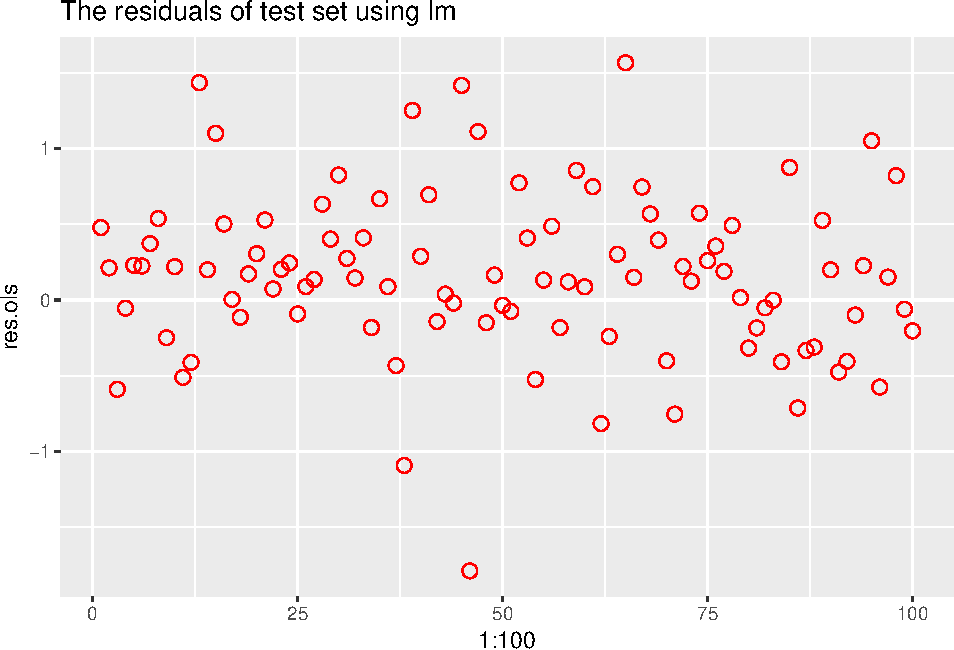
\includegraphics{FinalProjectForRegressionAnalysis_files/figure-latex/unnamed-chunk-36-1.pdf}

\subsubsection{使用主成分回归模型进行预测}

\begin{Shaded}
\begin{Highlighting}[]
\NormalTok{data2.test.pc <-}\StringTok{ }\KeywordTok{data.frame}\NormalTok{(}\KeywordTok{predict}\NormalTok{(y.pr, }\DataTypeTok{newdata =}\NormalTok{ data2.test))}
\NormalTok{ypred.log.pc <-}\StringTok{ }\KeywordTok{predict}\NormalTok{(pc.model, }\DataTypeTok{newdata =}\NormalTok{ data2.test.pc)}
\NormalTok{ypred.pc <-}\StringTok{ }\KeywordTok{exp}\NormalTok{(ypred.log.pc }\OperatorTok{*}\StringTok{ }\NormalTok{y.scale }\OperatorTok{+}\StringTok{ }\NormalTok{y.center)}
\NormalTok{res.pc <-}\StringTok{ }\NormalTok{y.log.test }\OperatorTok{-}\StringTok{ }\NormalTok{ypred.log.pc}
\NormalTok{mse.pc <-}\StringTok{ }\KeywordTok{mean}\NormalTok{(res.pc}\OperatorTok{^}\DecValTok{2}\NormalTok{)}
\NormalTok{mse.pc}
\end{Highlighting}
\end{Shaded}

\begin{verbatim}
## [1] 0.3156006
\end{verbatim}

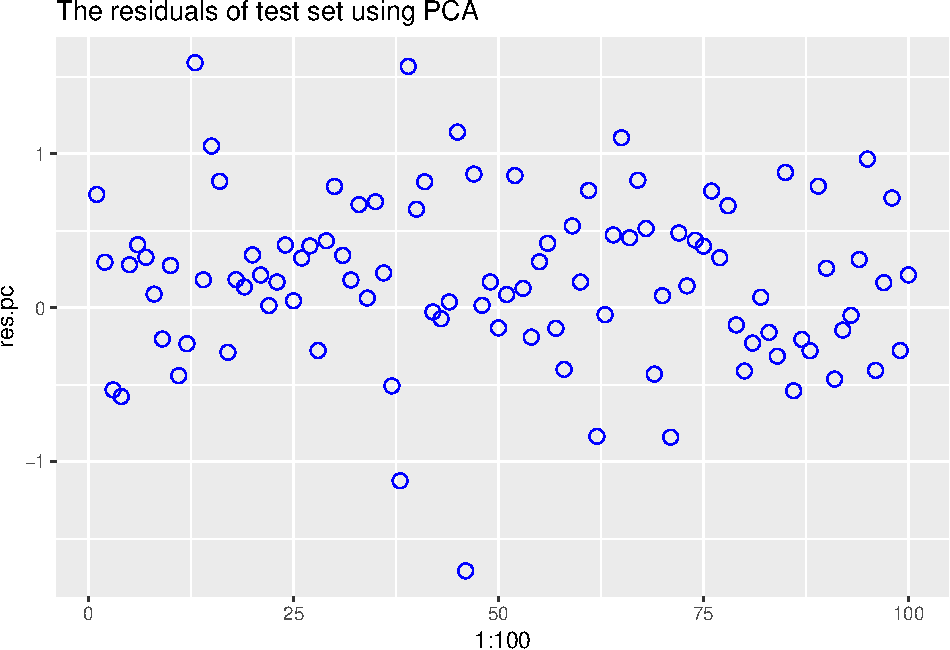
\includegraphics{FinalProjectForRegressionAnalysis_files/figure-latex/unnamed-chunk-37-1.pdf}

\subsubsection{使用岭回归模型进行预测}

\begin{Shaded}
\begin{Highlighting}[]
\NormalTok{ypred.log.ridge <-}\StringTok{ }\KeywordTok{rowSums}\NormalTok{(ridge.model}\OperatorTok{$}\NormalTok{coef }\OperatorTok{*}\StringTok{ }\NormalTok{data2.test)}
\NormalTok{ypred.ridge <-}\StringTok{ }\KeywordTok{exp}\NormalTok{(ypred.log.ridge }\OperatorTok{*}\StringTok{ }\NormalTok{y.scale }\OperatorTok{+}\StringTok{ }\NormalTok{y.center) }
\NormalTok{res.ridge <-}\StringTok{ }\NormalTok{y.log.test }\OperatorTok{-}\StringTok{ }\NormalTok{ypred.log.ridge}
\NormalTok{mse.ridge <-}\StringTok{ }\KeywordTok{mean}\NormalTok{(res.ridge}\OperatorTok{^}\DecValTok{2}\NormalTok{)}
\NormalTok{mse.ridge}
\end{Highlighting}
\end{Shaded}

\begin{verbatim}
## [1] 0.6553124
\end{verbatim}

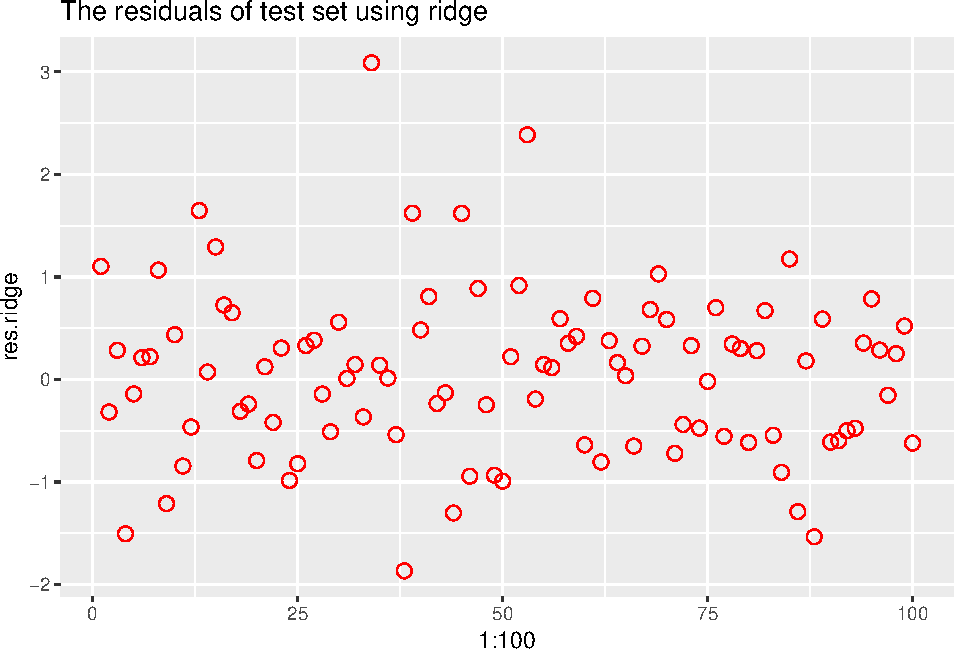
\includegraphics{FinalProjectForRegressionAnalysis_files/figure-latex/unnamed-chunk-38-1.pdf}








%
%==================================================================================================


\section{拓展}





%
%--------------------------------------------------------------------------------------------------
\subsection{Resample}\label{resample}

首先,在前面的报告中,可以看到我们并没有一次性将所有数据全部用于训练模型,因为否则我们将没有数据对我们的模型进行验证,从而评估模型的效果。前面的报告中,我们采用了一种最简单、也是最容易想到的方法,就是将整个数据集分成两部分,一部分用于训练,一部分用于验证,也就是训练集和测试集。

但是这种方法有两个弊端:首先是模型和参数的选择将很大依赖于对训练集和测试集的划分方法;此外,只使用了一部分数据进行模型的训练,而数据量越大模型效果通常会更好,所以模型的效果会受到一定的影响。

下面我们采用两种resample的方法,可以在一定程度上解决这个问题。

\subsubsection{Boostrap}\label{boostrap}

Boostrap是一种resample的方法,用于通过对替换的数据集进行重复多次采样来估计总体的统计数据,如均值、标准差,或者是总体的分布。

其实现的方式是这样子的:从训练集中有放回的均匀抽样,每个样本可以得到一个估计,这样一来,可以得到\(n\)个估计,也就可以估计出总体的分布。

\begin{Shaded}
\begin{Highlighting}[]
\KeywordTok{set.seed}\NormalTok{(}\DecValTok{123}\NormalTok{)}
\NormalTok{yname <-}\StringTok{ "z"}
\NormalTok{varnameList <-}\StringTok{ }\KeywordTok{names}\NormalTok{(step.model}\OperatorTok{$}\NormalTok{coefficients[}\OperatorTok{-}\DecValTok{1}\NormalTok{])}
\NormalTok{formu <-}\StringTok{ }\KeywordTok{as.formula}\NormalTok{(}\KeywordTok{paste}\NormalTok{(yname, }\KeywordTok{paste}\NormalTok{(}\StringTok{"~"}\NormalTok{, }\KeywordTok{paste}\NormalTok{(varnameList, }\DataTypeTok{collapse =} \StringTok{"+"}\NormalTok{))))}
\NormalTok{getRegr <-}\StringTok{ }\ControlFlowTok{function}\NormalTok{(data, idx) \{}
\NormalTok{  yname <-}\StringTok{ "z"}
\NormalTok{  varnameList <-}\StringTok{ }\KeywordTok{names}\NormalTok{(step.model}\OperatorTok{$}\NormalTok{coefficients[}\OperatorTok{-}\DecValTok{1}\NormalTok{])}
\NormalTok{  formu <-}\StringTok{ }\KeywordTok{as.formula}\NormalTok{(}\KeywordTok{paste}\NormalTok{(yname, }\KeywordTok{paste}\NormalTok{(}\StringTok{"~"}\NormalTok{, }\KeywordTok{paste}\NormalTok{(varnameList, }\DataTypeTok{collapse =} \StringTok{"+"}\NormalTok{))))}
\NormalTok{  bsFit <-}\StringTok{ }\KeywordTok{lm}\NormalTok{(formu, }\DataTypeTok{subset=}\NormalTok{idx, }\DataTypeTok{data=}\NormalTok{data)}
  \KeywordTok{coef}\NormalTok{(bsFit)}
\NormalTok{\}}
\NormalTok{nR <-}\StringTok{ }\DecValTok{1000}
\NormalTok{ols.model.boot <-}\StringTok{ }\KeywordTok{boot}\NormalTok{(data3.trans, }\DataTypeTok{statistic=}\NormalTok{getRegr, }\DataTypeTok{R=}\NormalTok{nR)}
\NormalTok{ols.model.boot}
\end{Highlighting}
\end{Shaded}

\begin{verbatim}
## ORDINARY NONPARAMETRIC BOOTSTRAP
## Call:
## boot(data = data3.trans, statistic = getRegr, R = nR)
## 
## Bootstrap Statistics :
##          original        bias    std. error
## t1* -5.815643e-15 -0.0021240787  0.02971774
## t2*  4.179040e-01 -0.0050539346  0.04656104
## t3*  3.532586e-01  0.0021085834  0.02780745
## t4*  2.241756e-01 -0.0021962496  0.04877214
## t5* -2.776035e-01  0.0006707451  0.03626421
## t6*  1.641309e-01  0.0011912137  0.03299041
## t7*  2.460243e-01  0.0060645856  0.04709809
## t8*  1.193177e-01  0.0034492458  0.03739097
\end{verbatim}

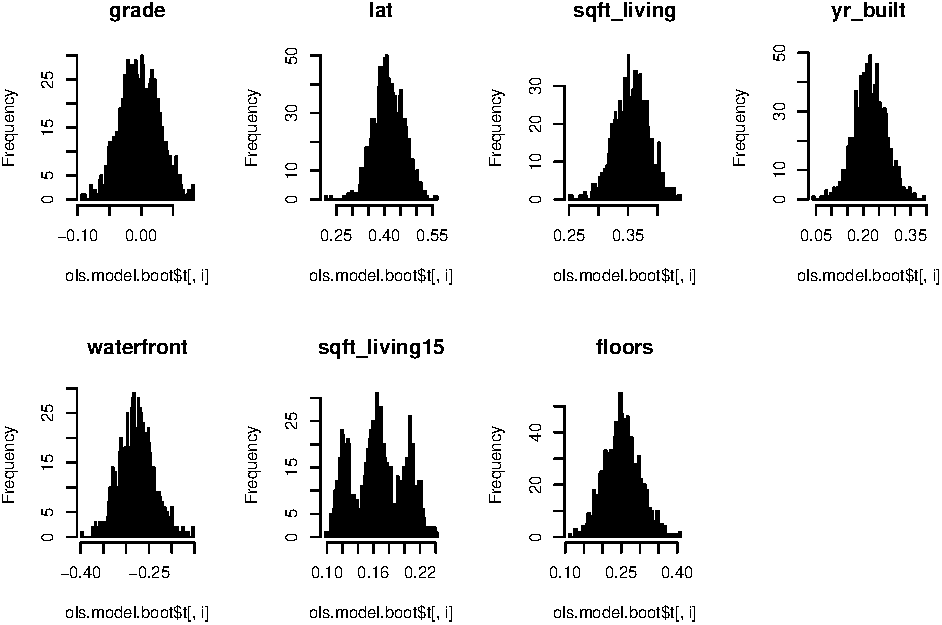
\includegraphics{FinalProjectForRegressionAnalysis_files/figure-latex/unnamed-chunk-39-1.pdf}

\subsubsection{Cross-Validation}\label{cross-validation}

为了解决上述问题,有人提出了Cross-Validation的方法。这是一种将样本数据切割成较小子集的方法,在部分子集中进行训练分析,其他子集则用来确认和验证,循环地将所有子集分析,可以得到一个较为稳健的估计。

\paragraph{Leave-One-Out
Cross-Validation}\label{leave-one-out-cross-validation}

Leave-One-Out
Cross-Validation(LOOCV)方法,也继承了上面的思路,但是不同的是,只用一个数据集作为验证集,其他数据作为训练集,并将此步骤重复N次(N为数据集的数量)。而最终的test均方误差就是这N次训练结果的平均值。
\[
CV_{(n)} = \frac{1}{n}\sum_{i = 1}^{n}MSE_i
\]

\begin{Shaded}
\begin{Highlighting}[]
\KeywordTok{set.seed}\NormalTok{(}\DecValTok{123}\NormalTok{)}
\NormalTok{yname <-}\StringTok{ "z"}
\NormalTok{varnameList <-}\StringTok{ }\KeywordTok{names}\NormalTok{(step.model}\OperatorTok{$}\NormalTok{coefficients[}\OperatorTok{-}\DecValTok{1}\NormalTok{])}
\NormalTok{formu <-}\StringTok{ }\KeywordTok{as.formula}\NormalTok{(}\KeywordTok{paste}\NormalTok{(yname, }\KeywordTok{paste}\NormalTok{(}\StringTok{"~"}\NormalTok{, }\KeywordTok{paste}\NormalTok{(varnameList, }\DataTypeTok{collapse =} \StringTok{"+"}\NormalTok{))))}
\NormalTok{ols.fit <-}\StringTok{ }\KeywordTok{glm}\NormalTok{(formu, }\DataTypeTok{data =}\NormalTok{ data3.trans)}
\NormalTok{cv.err <-}\StringTok{ }\KeywordTok{cv.glm}\NormalTok{(data3.trans, ols.fit)}
\NormalTok{cv.err}\OperatorTok{$}\NormalTok{delta}
\end{Highlighting}
\end{Shaded}

\begin{verbatim}
## [1] 0.1583323 0.1582820
\end{verbatim}

\paragraph{K-fold Cross-Validation}\label{k-fold-cross-validation}

另一种方法叫做K-fold
Cross-Validation,与LOOCV不同的是,每次的测试集不再只包含一个数据,而是k个数据,比如k
=
10,那么我们利用10-fold交叉验证的步骤,先将所有数据集分为10份,不重复地每次选取其中1份作为验证集,其他9份作为训练集训练模型,之后计算在该测试集的均方误差,最终将10次均方误差取评价。
\[
CV_{(k)} = \frac{1}{k}\sum_{i = 1}^{k}MSE_i
\] 不难看出,LOOCV是一种特殊的K-fold Cross-Validation(K = 1)。

\begin{Shaded}
\begin{Highlighting}[]
\KeywordTok{set.seed}\NormalTok{(}\DecValTok{123}\NormalTok{)}
\NormalTok{yname <-}\StringTok{ "z"}
\NormalTok{varnameList <-}\StringTok{ }\KeywordTok{names}\NormalTok{(step.model}\OperatorTok{$}\NormalTok{coefficients[}\OperatorTok{-}\DecValTok{1}\NormalTok{])}
\NormalTok{formu <-}\StringTok{ }\KeywordTok{as.formula}\NormalTok{(}\KeywordTok{paste}\NormalTok{(yname, }\KeywordTok{paste}\NormalTok{(}\StringTok{"~"}\NormalTok{, }\KeywordTok{paste}\NormalTok{(varnameList, }\DataTypeTok{collapse =} \StringTok{"+"}\NormalTok{))))}
\NormalTok{ols.fit <-}\StringTok{ }\KeywordTok{glm}\NormalTok{(formu, }\DataTypeTok{data =}\NormalTok{ data3.trans)}
\NormalTok{cv.err <-}\StringTok{ }\KeywordTok{cv.glm}\NormalTok{(data3.trans, ols.fit, }\DataTypeTok{K =} \DecValTok{10}\NormalTok{)}
\NormalTok{cv.err}\OperatorTok{$}\NormalTok{delta}
\end{Highlighting}
\end{Shaded}

\begin{verbatim}
## [1] 0.1583177 0.1573669
\end{verbatim}







%
%--------------------------------------------------------------------------------------------------
\subsection{Lasso, Ridge and Elastic
net}\label{lasso-ridge-and-elastic-net}

线性回归的最小二乘法,是为了使得目标函数最小化,即 \[
\min_\beta\{||Y-X\beta||^2\}
\]

Lasso, Ridge and Elastic
net这三个方法都是在回归过程中防止过拟合的出现的方法,在目标函数后添加正则项因子,
其中Lasso是使用\(L1-norm\)正则因子,即 \[
\min_\beta\{||Y-X\beta||^2 + \lambda ||\beta||_1\},\quad where\ ||\beta||_1 = \sum_i|\beta_i|,
\]

Ridge是使用\(L2-norm\)正则因子,即 \[
\min_\beta\{||Y-X\beta||^2 + \lambda ||\beta||_2\},\quad where\ ||\beta||_2 = \sum_i\beta_i^2,
\]

而Elastic net则是\(L1-norm\)和\(L2-norm\)的结合,即 \[
\min_\beta\{||Y-X\beta||^2 + \lambda[\alpha||\beta||_1 + (1-\alpha) ||\beta||_2 ] \}.
\]

下面将结合这三种方法和Cross-Validation的方法进行分析。

\subsubsection{训练模型}

我们使用的是glmnet这个包中的glmnet函数,其中的alpha参数也就是上述Elastic
net中的\(\alpha\)。注意到\(\alpha = 1\)是Lasso模型,\(\alpha = 0\)是Ridge模型。

\begin{Shaded}
\begin{Highlighting}[]
\NormalTok{fit.lasso <-}\StringTok{ }\KeywordTok{glmnet}\NormalTok{(x.train, y.train, }\DataTypeTok{family=}\StringTok{"gaussian"}\NormalTok{, }\DataTypeTok{alpha=}\DecValTok{1}\NormalTok{)}
\NormalTok{fit.ridge <-}\StringTok{ }\KeywordTok{glmnet}\NormalTok{(x.train, y.train, }\DataTypeTok{family=}\StringTok{"gaussian"}\NormalTok{, }\DataTypeTok{alpha=}\DecValTok{0}\NormalTok{)}
\NormalTok{fit.elnet <-}\StringTok{ }\KeywordTok{glmnet}\NormalTok{(x.train, y.train, }\DataTypeTok{family=}\StringTok{"gaussian"}\NormalTok{, }\DataTypeTok{alpha=}\NormalTok{.}\DecValTok{5}\NormalTok{)}

\CommentTok{# Plot solution paths:}
\end{Highlighting}
\end{Shaded}

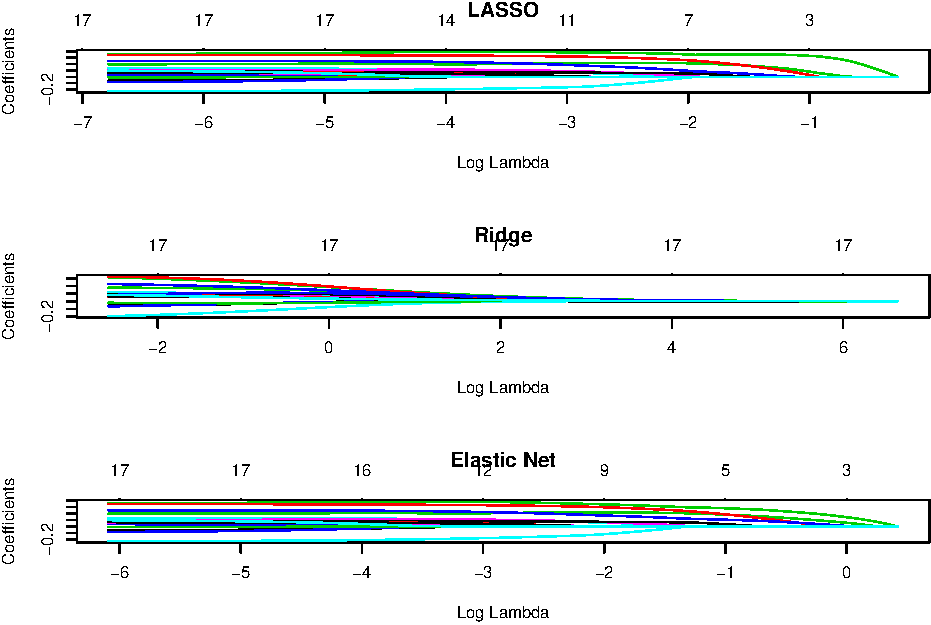
\includegraphics{FinalProjectForRegressionAnalysis_files/figure-latex/unnamed-chunk-42-1.pdf}

下面使用10-Fold
Cross-Validation对\(\alpha = 0, 0.1, \dots, 0.9, 1.0\)进行分析。

\begin{Shaded}
\begin{Highlighting}[]
\KeywordTok{set.seed}\NormalTok{(}\DecValTok{123}\NormalTok{)}
\ControlFlowTok{for}\NormalTok{ (i }\ControlFlowTok{in} \DecValTok{0}\OperatorTok{:}\DecValTok{10}\NormalTok{) \{}
  \KeywordTok{assign}\NormalTok{(}\KeywordTok{paste}\NormalTok{(}\StringTok{"fit"}\NormalTok{, i, }\DataTypeTok{sep=}\StringTok{""}\NormalTok{), }\KeywordTok{cv.glmnet}\NormalTok{(x.train, y.train, }
         \DataTypeTok{type.measure=}\StringTok{"mse"}\NormalTok{,  }\DataTypeTok{alpha=}\NormalTok{i}\OperatorTok{/}\DecValTok{10}\NormalTok{,}\DataTypeTok{family=}\StringTok{"gaussian"}\NormalTok{))}
\NormalTok{\}}
\end{Highlighting}
\end{Shaded}

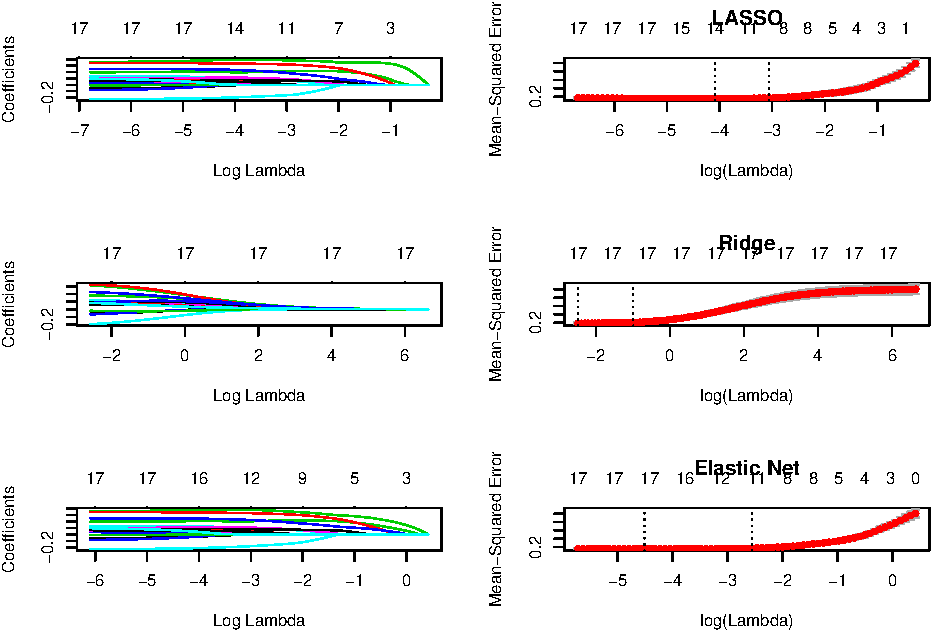
\includegraphics{FinalProjectForRegressionAnalysis_files/figure-latex/unnamed-chunk-43-1.pdf}

\subsubsection{预测}\label{-1}

\begin{Shaded}
\begin{Highlighting}[]
\NormalTok{x.test <-}\StringTok{ }\KeywordTok{as.matrix}\NormalTok{(data2.test)}
\NormalTok{y.test <-}\StringTok{ }\NormalTok{data.test}\OperatorTok{$}\NormalTok{price}
\NormalTok{y.log.test <-}\StringTok{ }\NormalTok{(}\KeywordTok{log}\NormalTok{(y.test) }\OperatorTok{-}\StringTok{ }\NormalTok{y.center) }\OperatorTok{/}\StringTok{ }\NormalTok{y.scale}
\NormalTok{yhat0 <-}\StringTok{ }\KeywordTok{predict}\NormalTok{(fit0, }\DataTypeTok{s=}\NormalTok{fit0}\OperatorTok{$}\NormalTok{lambda.1se, }\DataTypeTok{newx=}\NormalTok{x.test)}
\NormalTok{yhat1 <-}\StringTok{ }\KeywordTok{predict}\NormalTok{(fit1, }\DataTypeTok{s=}\NormalTok{fit1}\OperatorTok{$}\NormalTok{lambda.1se, }\DataTypeTok{newx=}\NormalTok{x.test)}
\NormalTok{yhat2 <-}\StringTok{ }\KeywordTok{predict}\NormalTok{(fit2, }\DataTypeTok{s=}\NormalTok{fit2}\OperatorTok{$}\NormalTok{lambda.1se, }\DataTypeTok{newx=}\NormalTok{x.test)}
\NormalTok{yhat3 <-}\StringTok{ }\KeywordTok{predict}\NormalTok{(fit3, }\DataTypeTok{s=}\NormalTok{fit3}\OperatorTok{$}\NormalTok{lambda.1se, }\DataTypeTok{newx=}\NormalTok{x.test)}
\NormalTok{yhat4 <-}\StringTok{ }\KeywordTok{predict}\NormalTok{(fit4, }\DataTypeTok{s=}\NormalTok{fit4}\OperatorTok{$}\NormalTok{lambda.1se, }\DataTypeTok{newx=}\NormalTok{x.test)}
\NormalTok{yhat5 <-}\StringTok{ }\KeywordTok{predict}\NormalTok{(fit5, }\DataTypeTok{s=}\NormalTok{fit5}\OperatorTok{$}\NormalTok{lambda.1se, }\DataTypeTok{newx=}\NormalTok{x.test)}
\NormalTok{yhat6 <-}\StringTok{ }\KeywordTok{predict}\NormalTok{(fit6, }\DataTypeTok{s=}\NormalTok{fit6}\OperatorTok{$}\NormalTok{lambda.1se, }\DataTypeTok{newx=}\NormalTok{x.test)}
\NormalTok{yhat7 <-}\StringTok{ }\KeywordTok{predict}\NormalTok{(fit7, }\DataTypeTok{s=}\NormalTok{fit7}\OperatorTok{$}\NormalTok{lambda.1se, }\DataTypeTok{newx=}\NormalTok{x.test)}
\NormalTok{yhat8 <-}\StringTok{ }\KeywordTok{predict}\NormalTok{(fit8, }\DataTypeTok{s=}\NormalTok{fit8}\OperatorTok{$}\NormalTok{lambda.1se, }\DataTypeTok{newx=}\NormalTok{x.test)}
\NormalTok{yhat9 <-}\StringTok{ }\KeywordTok{predict}\NormalTok{(fit9, }\DataTypeTok{s=}\NormalTok{fit9}\OperatorTok{$}\NormalTok{lambda.1se, }\DataTypeTok{newx=}\NormalTok{x.test)}
\NormalTok{yhat10 <-}\StringTok{ }\KeywordTok{predict}\NormalTok{(fit10, }\DataTypeTok{s=}\NormalTok{fit10}\OperatorTok{$}\NormalTok{lambda.1se, }\DataTypeTok{newx=}\NormalTok{x.test)}

\NormalTok{mse0 <-}\StringTok{ }\KeywordTok{mean}\NormalTok{((y.log.test }\OperatorTok{-}\StringTok{ }\NormalTok{yhat0)}\OperatorTok{^}\DecValTok{2}\NormalTok{)}
\NormalTok{mse1 <-}\StringTok{ }\KeywordTok{mean}\NormalTok{((y.log.test }\OperatorTok{-}\StringTok{ }\NormalTok{yhat1)}\OperatorTok{^}\DecValTok{2}\NormalTok{)}
\NormalTok{mse2 <-}\StringTok{ }\KeywordTok{mean}\NormalTok{((y.log.test }\OperatorTok{-}\StringTok{ }\NormalTok{yhat2)}\OperatorTok{^}\DecValTok{2}\NormalTok{)}
\NormalTok{mse3 <-}\StringTok{ }\KeywordTok{mean}\NormalTok{((y.log.test }\OperatorTok{-}\StringTok{ }\NormalTok{yhat3)}\OperatorTok{^}\DecValTok{2}\NormalTok{)}
\NormalTok{mse4 <-}\StringTok{ }\KeywordTok{mean}\NormalTok{((y.log.test }\OperatorTok{-}\StringTok{ }\NormalTok{yhat4)}\OperatorTok{^}\DecValTok{2}\NormalTok{)}
\NormalTok{mse5 <-}\StringTok{ }\KeywordTok{mean}\NormalTok{((y.log.test }\OperatorTok{-}\StringTok{ }\NormalTok{yhat5)}\OperatorTok{^}\DecValTok{2}\NormalTok{)}
\NormalTok{mse6 <-}\StringTok{ }\KeywordTok{mean}\NormalTok{((y.log.test }\OperatorTok{-}\StringTok{ }\NormalTok{yhat6)}\OperatorTok{^}\DecValTok{2}\NormalTok{)}
\NormalTok{mse7 <-}\StringTok{ }\KeywordTok{mean}\NormalTok{((y.log.test }\OperatorTok{-}\StringTok{ }\NormalTok{yhat7)}\OperatorTok{^}\DecValTok{2}\NormalTok{)}
\NormalTok{mse8 <-}\StringTok{ }\KeywordTok{mean}\NormalTok{((y.log.test }\OperatorTok{-}\StringTok{ }\NormalTok{yhat8)}\OperatorTok{^}\DecValTok{2}\NormalTok{)}
\NormalTok{mse9 <-}\StringTok{ }\KeywordTok{mean}\NormalTok{((y.log.test }\OperatorTok{-}\StringTok{ }\NormalTok{yhat9)}\OperatorTok{^}\DecValTok{2}\NormalTok{)}
\NormalTok{mse10 <-}\StringTok{ }\KeywordTok{mean}\NormalTok{((y.log.test }\OperatorTok{-}\StringTok{ }\NormalTok{yhat10)}\OperatorTok{^}\DecValTok{2}\NormalTok{)}
\NormalTok{mse_}\DecValTok{1}\NormalTok{ =}\StringTok{ }\KeywordTok{c}\NormalTok{(mse0,mse1,mse2,mse3,mse4,mse5,mse6,mse7,mse8,mse9,mse10)}
\end{Highlighting}
\end{Shaded}

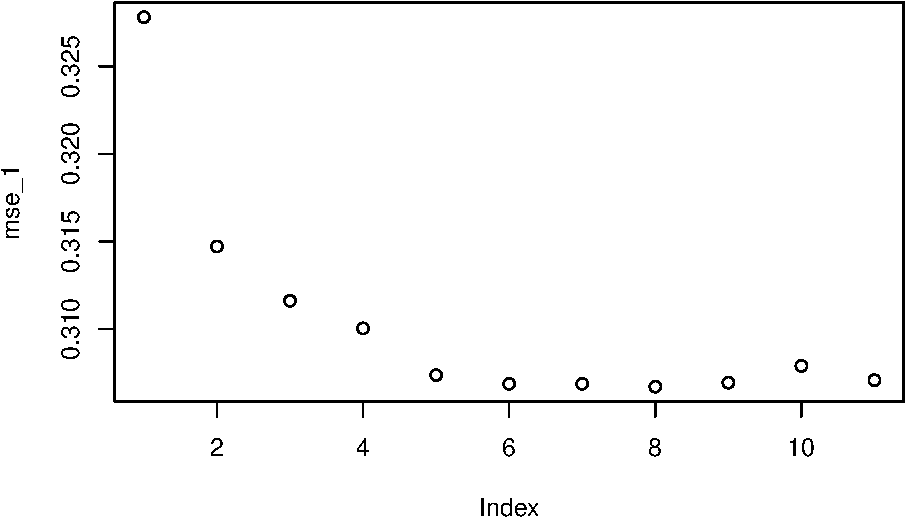
\includegraphics{FinalProjectForRegressionAnalysis_files/figure-latex/unnamed-chunk-44-1.pdf}

我们可以看到,当\(\alpha = 0.7\)的时候,均方误差最小。

\begin{Shaded}
\begin{Highlighting}[]
\KeywordTok{which}\NormalTok{(mse_}\DecValTok{1} \OperatorTok{==}\StringTok{ }\KeywordTok{min}\NormalTok{(mse_}\DecValTok{1}\NormalTok{))}
\end{Highlighting}
\end{Shaded}

\begin{verbatim}
## [1] 8
\end{verbatim}


\end{document}
